\documentclass[11pt]{article} % do not change this line
\input{BigDataStyle.txt}      % do not change this line
\usepackage{amsmath,amsfonts,amssymb,amsthm,latexsym,graphicx,float,subcaption,geometry,booktabs, multicol}
\usepackage[linesnumbered,ruled]{algorithm2e}
\usepackage[toc,page]{appendix}
\emergencystretch=5mm
\tolerance=400
\allowdisplaybreaks[4]

%\setlength{\parindent}{2em}
\setlength{\parskip}{0.5em}

\theoremstyle{plain}
\newtheorem{theorem}{Theorem}[section]
\newtheorem{proposition}[theorem]{Proposition}
\newtheorem{corollary}[theorem]{Corollary}
\newtheorem{lemma}[theorem]{Lemma}
\newtheorem{problem}[theorem]{Problem}

\theoremstyle{definition}
\newtheorem*{remark}{Remark}

\title{Sequence-to-Sequence Model for Signal Analysis}
\author{Timothy Wong}

\newcommand{\Programme}{Data Science and Analytics}
% Computational Finance students: uncomment the next line
%\twodepartmentstrue

\begin{document}
\maketitle

\declaration

\begin{abstract}

Large-scale industrial processes are often monitored by many sensors. This study proposes using artificial neural network based approach to capture complex temporal patterns across multiple sensors. To achieve this, sequence-to-sequence model can be modified into an autoencoder by aligning the input and output sequences. The model's encoder summarises the input into a vector which can be used to represent meaningful features. When consecutively drawn samples are fed to the model, the summary information varies in a way which reflects the change in complex temporal patterns. This information is analysed further by applying visualisation and clustering techniques.

We illustrated the application of the proposed algorithm with a proprietary dataset collected from an industrial scale two-stage compression train. This study also experimented various hyperparameters and studied their effects on the model's properties. This proposed method can be generalised to any multi-sensor multi-state processes for signal analysis purpose.

\end{abstract}

\section{Introduction}

Modern industrial processes are often monitored by a large array of sensors. Vital data is usually displayed on the equipment panel or streamed to computerised real-time dashboards in the control room. Automated rule-based systems are commonly in place to monitor streams of real-time sensor readings. For instance, warning alarm can be triggered if vital sensor reaches a pre-set threshold value. This allows operators to intervene in time and apply corrective actions appropriately. However, the process state may continue to worsen if manual intervention fails to resolve the problem. This would eventually trigger automated shutdown when the process reached the critical state. The intention is to guarantee safety and protect the equipment from any further damage. In many real-world scenarios, operators need to conduct detailed safety inspection before restarting the production process. Unplanned shutdown inevitably causes loss production, it can also lead to substandard product or even safety breach.

Machine learning techniques can be used to analyse signal data in an on-line scenario. It is found that neural network algorithms can be used to handle streams of sensor measurements natively and learn complex patterns intelligently over time. Using a large-scale gas production process as example, this study suggests that the proposed approach can generate meaningful diagnostic measurements using real-time sensor data. These measurements can then be used to identify abnormal patterns or substantial change in the underlying process state, thus enabling operators to anticipate and mitigate problems.

\subsection{Application Area}

This application is centred on a two-stage gas compression train at a natural gas terminal. It receives unprocessed gas from offshore platform via subsurface pipeline. The incoming gas reaches the compressor at a variable, naturally-occurring pressure. This implies that the gas pressure needs to be regulated and increased to an appropriate level before feeding it to other downstream processes. The compression subsystem has many components as illustrated in the process diagram in figure \ref{fig:process_diagram}.

\begin{figure}[h]
	\centering
	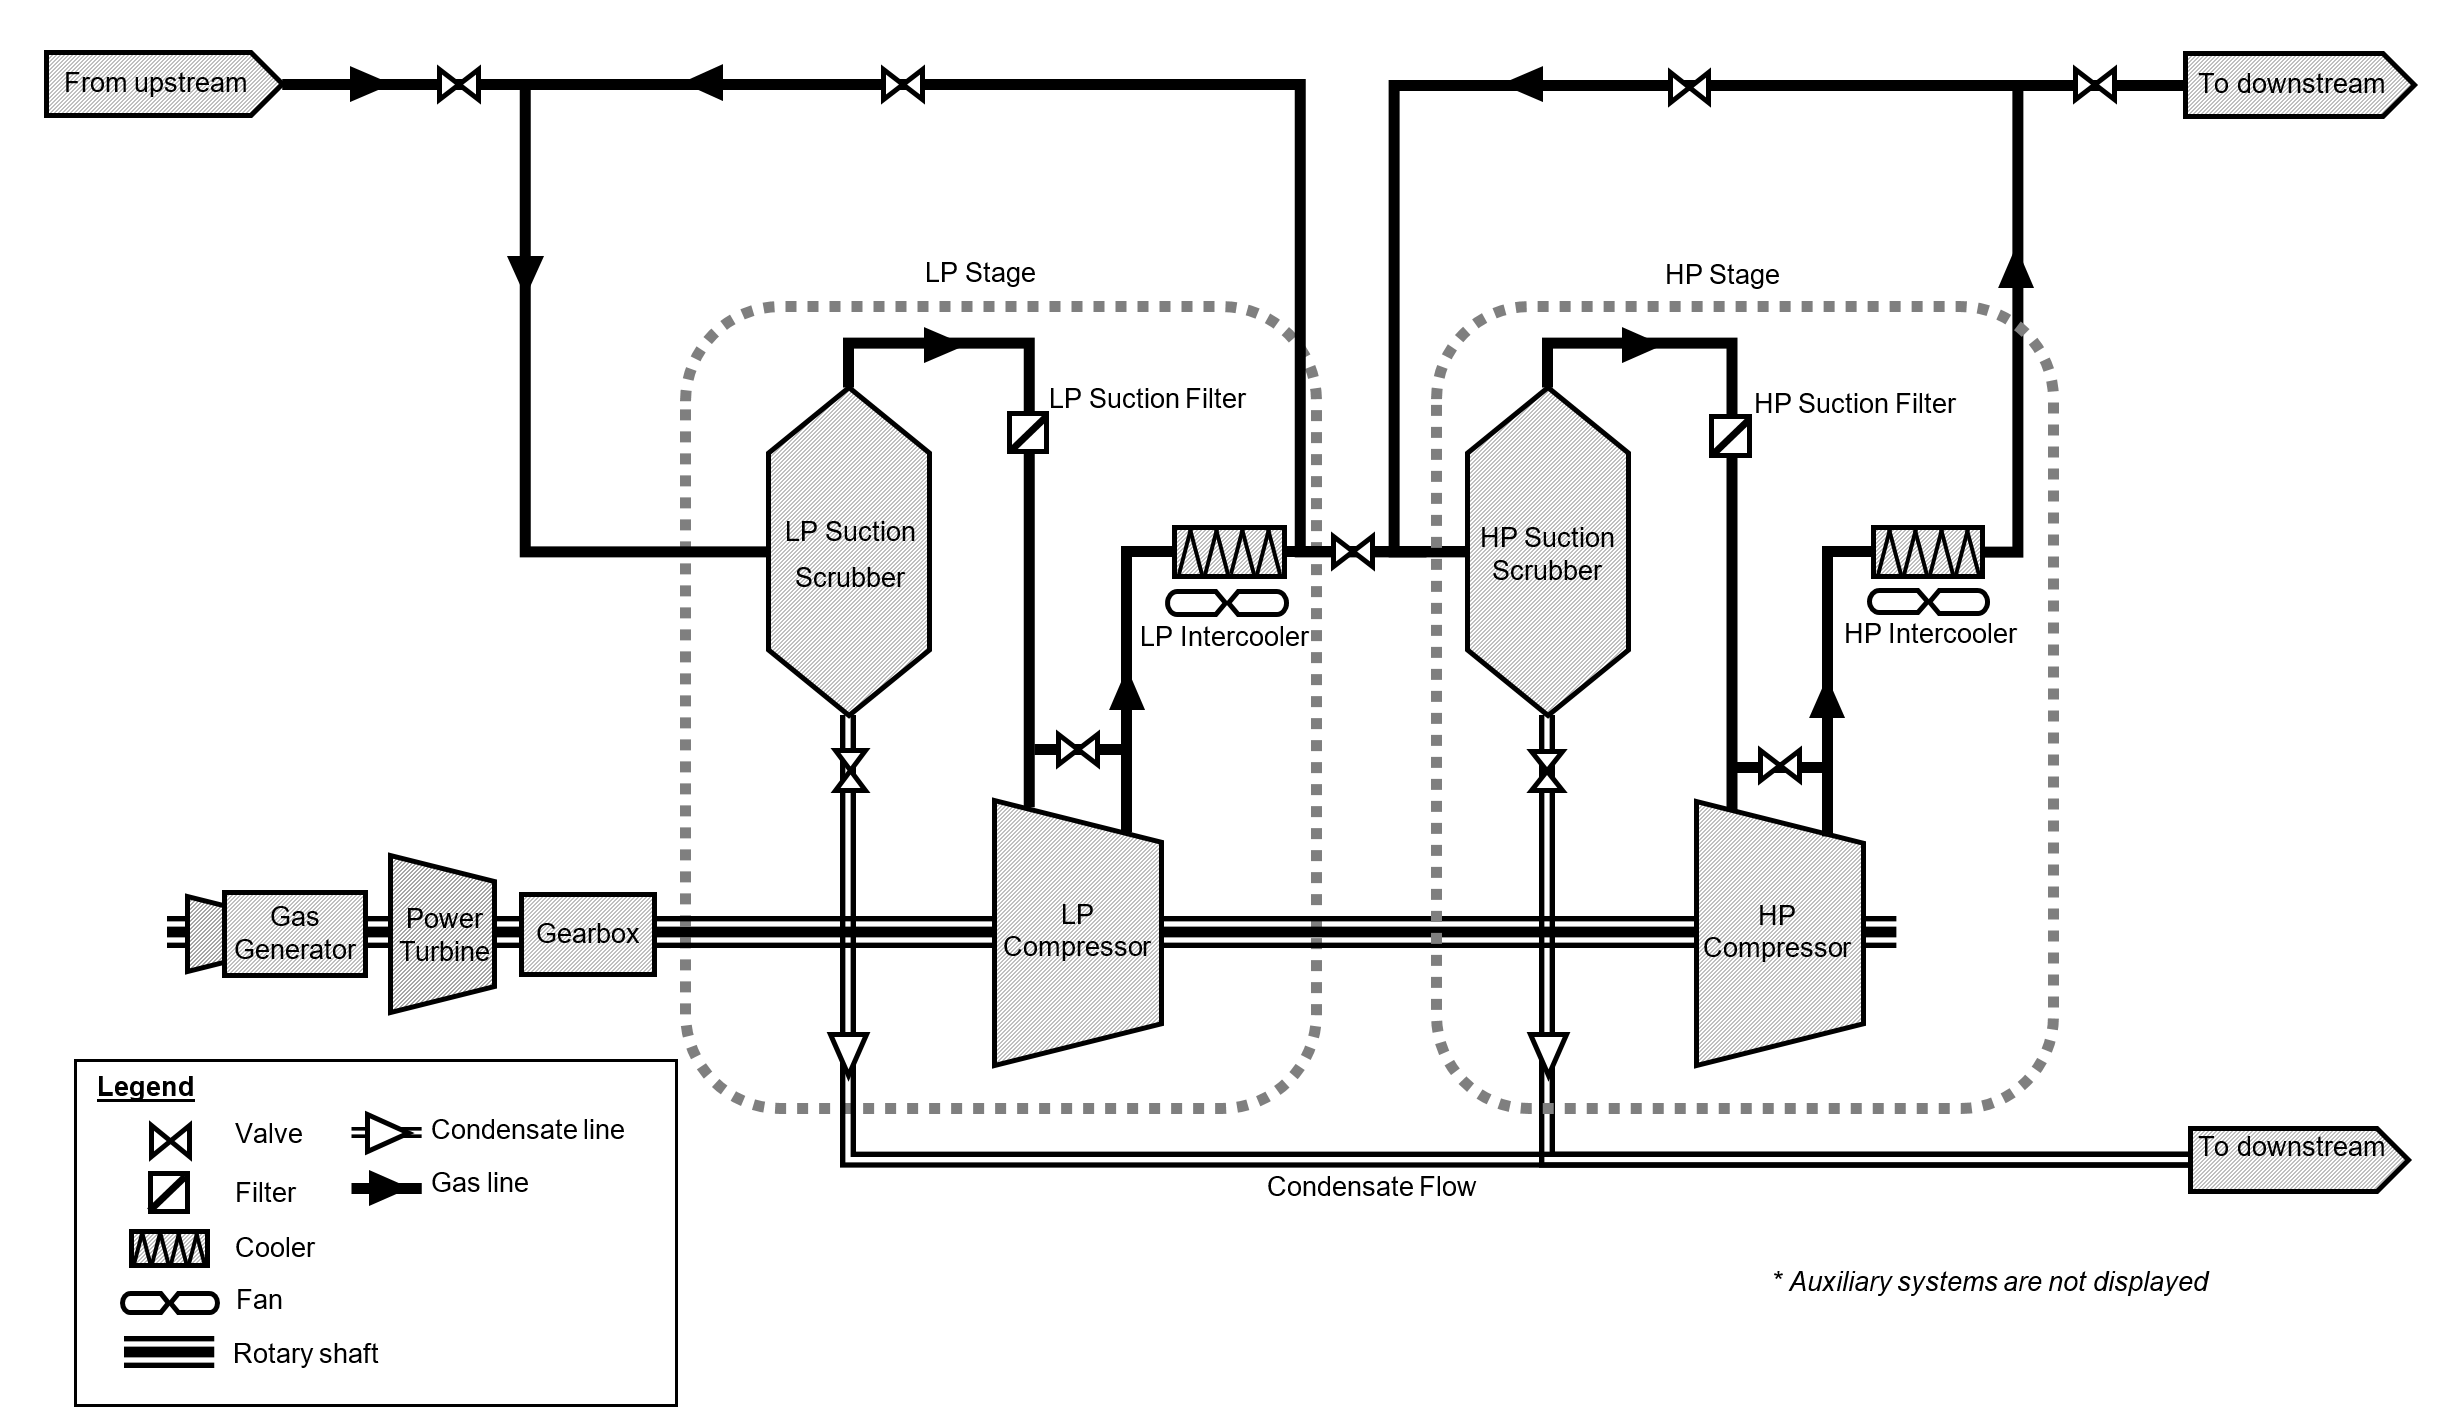
\includegraphics[width=1\textwidth]{process_diagram.PNG}
	\caption{Simplified process diagram showing a two-stage gas compression train}
	\label{fig:process_diagram}
\end{figure}

The compression train uses two centrifugal compressors connected in serial to raise the gas pressure in separate stages. At first, the incoming gas flows through a suction scrubber to remove condensate in the Low Pressure (LP) stage. Dry gas exits the scrubber through the top outlet and passes through a gas filter. The LP compressor receives gas through the suction inlet and raises the gas pressure to an intermediate level. The compressed gas from LP stage leaves via the discharge outlet and the temperature is reduced at the intercooler afterwards. Gas then goes through the High Pressure (HP) stage which raises the pressure further to a higher level through similar configuration. Both LP and HP stages are driven by an aeroderivative gas generator on a single shaft.

Sensors are attached to various parts of the compression train to monitor the production process. Vital statistics like temperature, pressure, rotary speed, vibration… etc., are recorded at different locations. Several key components are notoriously vulnerable to tripping. For example, lack of lubrication would cause high vibration which eventually trips the entire compression train. Alternatively, discharging gas at unstable pressure may risk damaging downstream equipment, etc.

\subsection{Problem Formulation}

As previously mentioned, simple rule-based system can be used to highlight issues (e.g. thresholding) in production process. However, complex patterns over time are hard to describe explicitly especially when it involves a group of sensors. The intuition of the proposed diagnostic measurement is to address this problem by considering the whole process state as a multidimensional entity which varies over time.

Each stream of sensor measurement is basically a set of real values \(\mathbb{R}\) received in a time-ordered fashion. When this concept is extended to a process with \(P\) sensors, the process can therefore be expressed as a time-ordered multidimensional vector \( \{ \mathbb{R}_t^P:t\in [1,T] \} \).

Neural network offers a way to handle the high-dimensional data natively which will be outlined in the later sections. The fundamental objective of this study is to use these techniques to analyse multidimensional time series data and understand the change of the underlying process state. Warnings can be triggered by process state transition or substantial deviation is observed. Although the discussion of the proposed approach is focused on the natural gas terminal use case, it can be further extended to any multi-sensor multi-state processes.

\newpage
\section{Data Preprocessing}

Streams of sensor measurements were recorded in a production database system. A batch extract of all sensor readings was obtained as a collection of comma-separated text files.

\subsection{Downsampling}

The raw sensor data was recorded continuously at very granular level. The interval between records can range between \(1\) to \(10\) seconds depending on the process configuration at the time. Shorter time interval obviously gives a more detailed view of the process. However, problems arise when successive sensor values are not guaranteed to have fixed interval in between them. Although time series analysis accepts time-order data, it straightly requires successive observations to be separated by equal time interval. This implies that there is a need to standardise the raw sensor dataset in order to create equally-spaced data for further analysis.

In many signal processing applications, windowing approach is used to convert high-frequency data with irregularly-interval into equally-spaced time series. Through this preprocessing step, the size of the data is reduced therefore it is also called downsampling. We will discuss how this technique can be applied to preprocess the data.

\subsubsection{Tumbling Time Window}

The simplest way to downsample the raw data is to apply tumbling time window along the timeline of the raw data. Windows of equal sizes are imposed successively without any gap or overlapping in between. For any given window of size \(W\), a sampling function evaluate all the member vectors and returns a single vector as the representative sample of the current window. Commonly used sampling functions include simple arithmetic averaging, taking median value, or returning the last member\footnote{Sorting all the input vectors chronologically and return the most recent.}. The figure below offers a graphical illustration of tumbling time window which returns the last value within any given time window.

\begin{figure}[H]
	\centering
	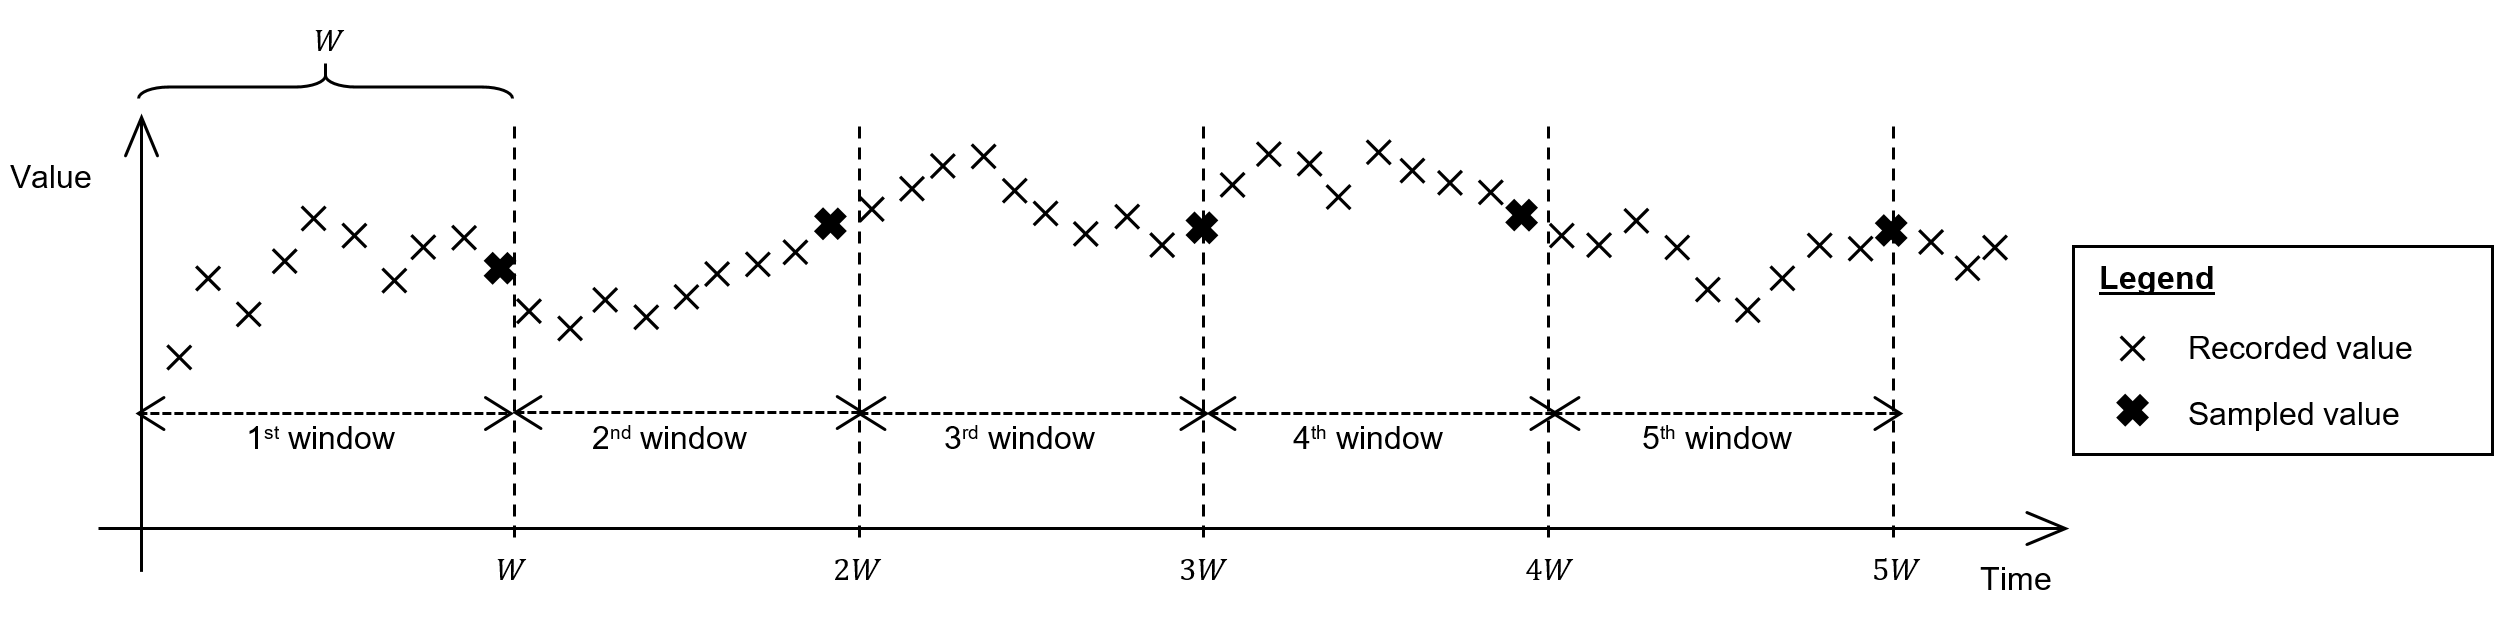
\includegraphics[width=1\textwidth]{tumbling_time_window.PNG}
	\caption{Graphical illustration of tumbling time window}
	\label{fig:tumbling_time_window}
\end{figure}


\subsubsection{Sliding Time Window}

An alternative way to downsample the raw data is to use the sliding time window approach. It is basically a special case of the tumbling windows approach where overlapping between successive time window is allowed. The parameter \(W\) determines the window size, while the overlapping size is controlled by the parameter \(k\). Once the windows are established, a sampling function is applied to all member vectors of the window and one representative vector is returned as the downsampled sequence. 

\begin{figure}[H]
	\centering
	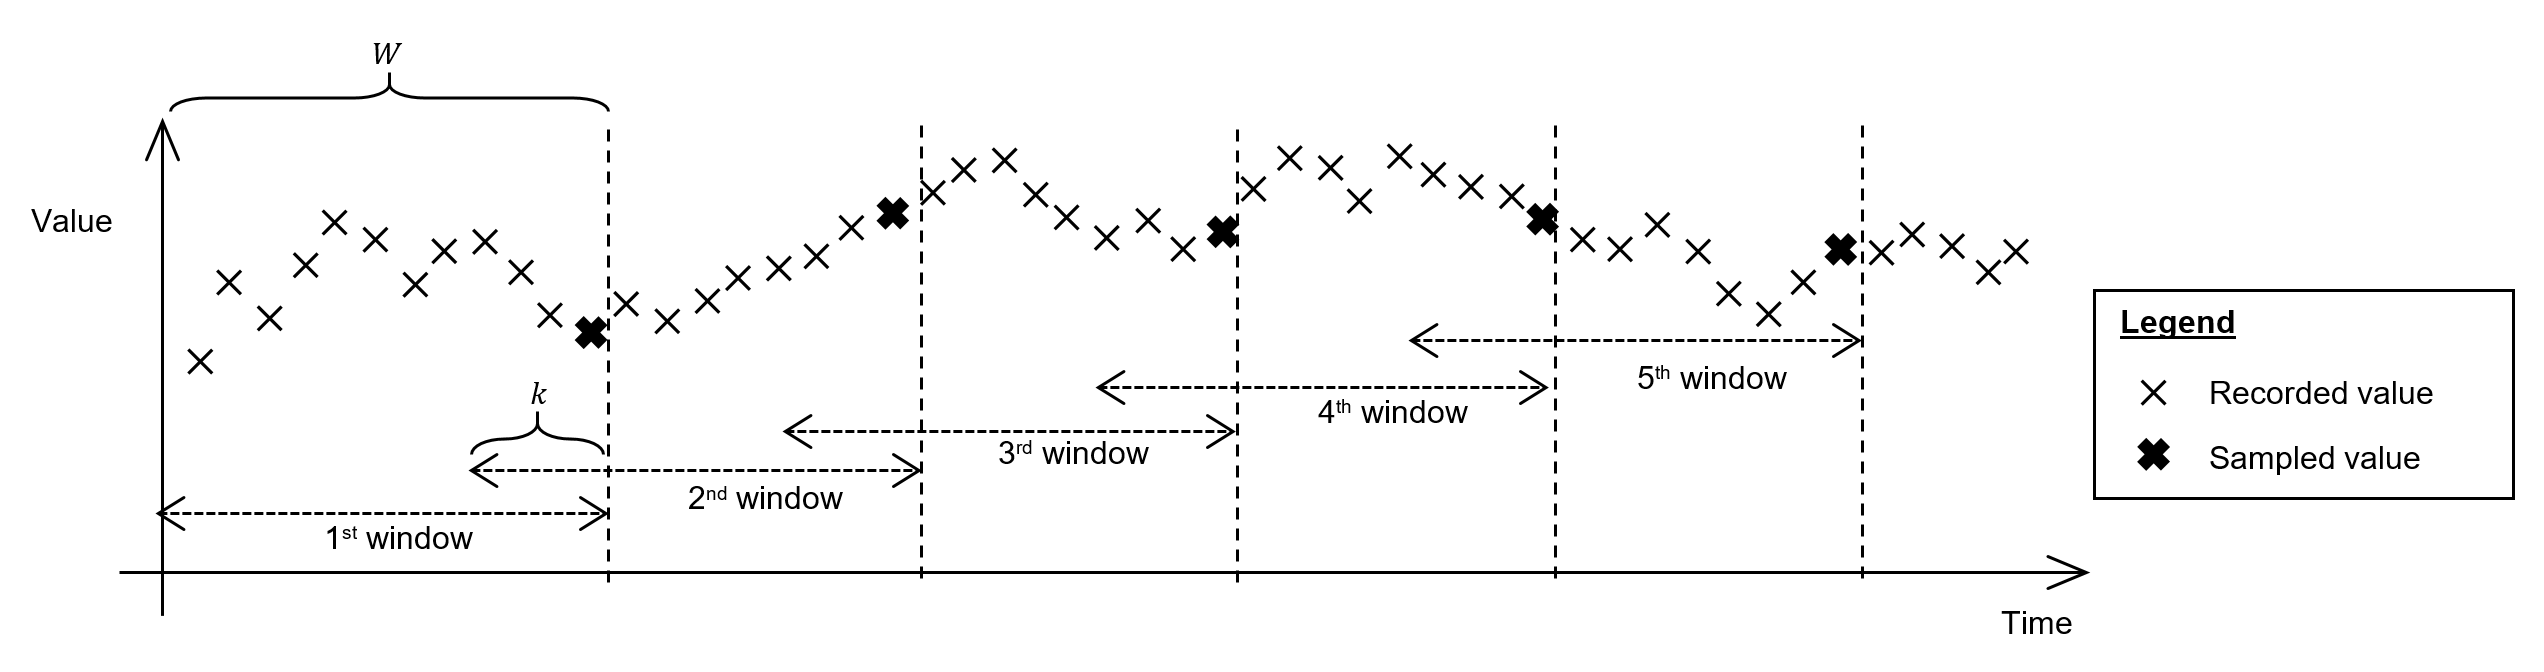
\includegraphics[width=1\textwidth]{sliding_time_window.PNG}
	\caption{Graphical illustration of sliding time window}
	\label{fig:sliding_time_window}
\end{figure}


\subsection{Subsetting}

Once the downsampled data is prepared, successive sensor records are guaranteed to have equal time interval in between them. Yet, we must bear in mind that the production process may suffer outage despite valid sensor reading are still continuously recorded. Besides, the production equipment may have been reconfigured or modified during downtime. In light of these reasons, data recorded over known outage periods are discarded from the training dataset. In addition, short periods are discarded form the dataset as they usually indicate safety testing rather than actual production process. The following figure summarises the downsampling and subsetting stage.

\begin{figure}[H]
	\centering
	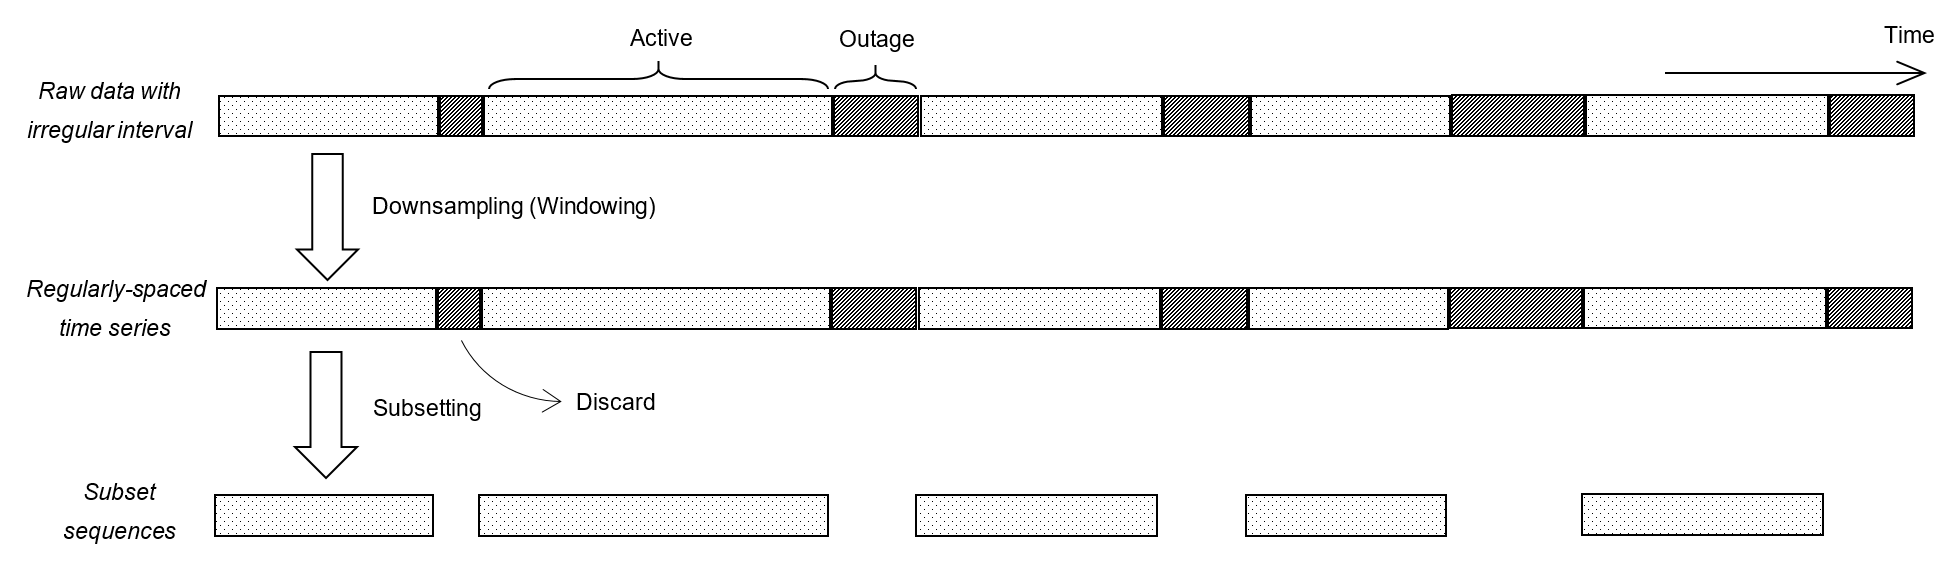
\includegraphics[width=1\textwidth]{preprocessing.PNG}
	\caption{Data preprocessing stages. Raw sensor measurements were standardised into regularly-spaced time series data using the windowing approach. Afterwards, known outage periods were discarded from the dataset. }
	\label{fig:preprocessing}
\end{figure}




\newpage
\section{Methods}

To begin with, artificial neural network (ANN) is a type of algorithm inspired by biological neurons. It consists of a collection of artificial neurons which are capable of processing incoming signals through a series of connected units. As early as 1943, McCulloch \& Pitts \cite{mcculloch} presented an artificial neuron which mimics firing of biological neurons. The neuron excites if the weighted sum of binary inputs exceeds certain threshold. The neuron’s output is also binary in nature which feeds through a network. A decade later, Rosenblatt \cite{rosenblatt} further outlined ANN as a supervised learning algorithm. He developed the revolutionary Perceptron device which performs pattern classification tasks using learnable weights. The device has neurons arranged in a single layer which compute the weighted sum of the inputs and decide whether to fire. 

Modern ANNs are essentially very similar to the ones described above. We can illustrate this using an ANN which takes an input vector \(\mathbb{R}^P\) and learns the output vector \(\mathbb{R}^K\) (i.e. ANN performs vector mapping function \(f: \mathbb{R}^P\rightarrow\mathbb{R}^K \)). Figure \ref{fig:ann} below shows an ANN with a single hidden layer of \(H\) neurons. Each \(h\)\textsuperscript{th} neuron where \(h=1,...,H\) applies a weight \(w_{p,h}\) on the \(p\)\textsuperscript{th} input dimension of the vector \(\mathbb{R}^P\) where \(p\in{1,2,3,...,P}\) and the weighted sum of input is adjusted with a bias \(b_h\) as shown in equation \ref{weightedinput}. The bias-adjusted weighted input \(x_h\) then feeds through a non-linear function in a process called activation \eqref{activation}. 

\begin{figure}[H]
	\centering
	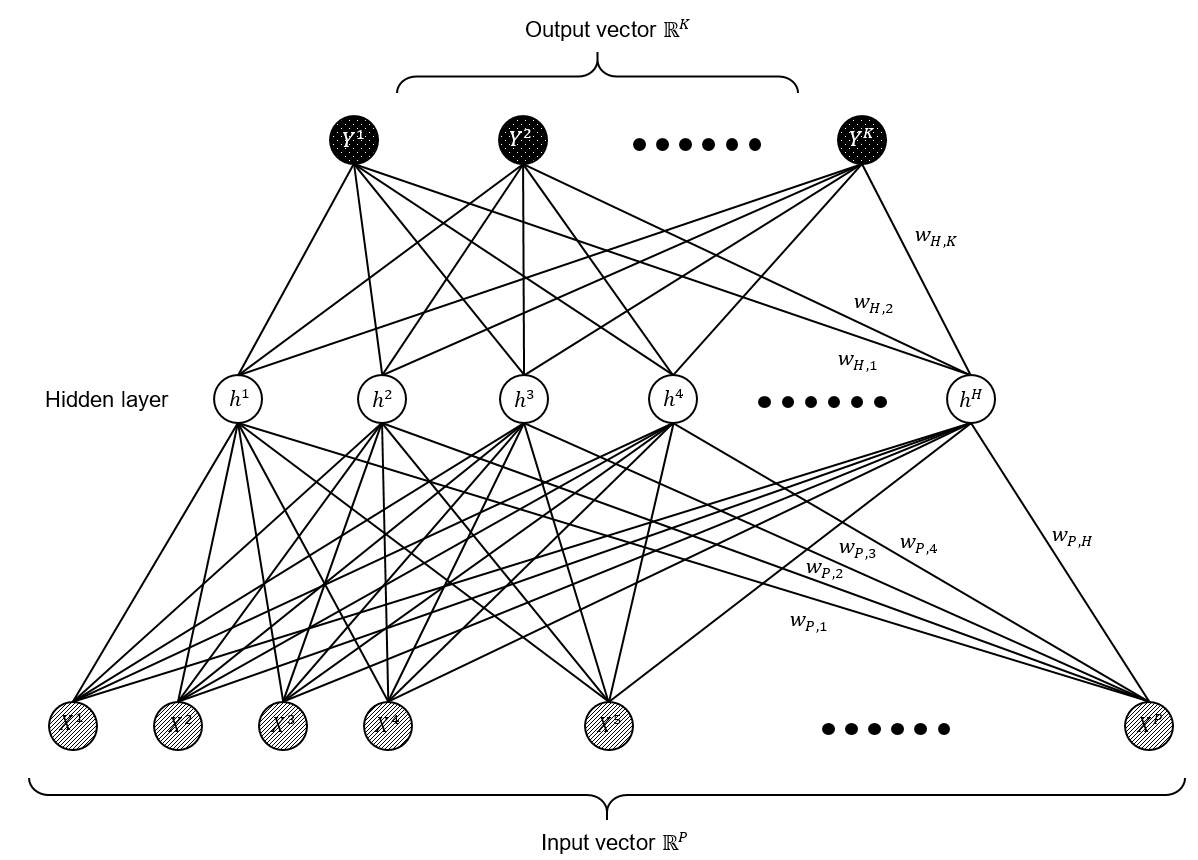
\includegraphics[width=0.65\textwidth]{ann.PNG}
	\caption{A simple forward-feeding artificial neural network (FNN) with one hidden layer. The input vector \(\mathbb{R}^P\) feeds through the input layer of \(P\) neurons. Each neuron in the hidden layer computes the weighted sum and bias adjustment as in equation \ref{weightedinput} and then it is activated as in equation \ref{activation}.}
	\label{fig:ann}
\end{figure}

Weighted sum and bias adjustment
\begin{equation}
\label{weightedinput}
x_h=b_h+\sum_{p=1}^{P} w_{p,h}X_p , h=1,...,H
\end{equation}

Activation
\begin{equation}
\label{activation}
h_h=f(x_h), h=1,...,H
\end{equation}

ANNs with information flowing in one direction (i.e. without loops) is called forward-feeding neural network (FNN). Such typology can be extended to multiple hidden layers, thus forming a multilayer perceptron (MLP) network.

\subsection{Recurrent Neural Network}

The objective of traditional ANNs is to map an input vector to an output vector through non-linear modelling. Ordering of the observations is immaterial in the sense that the models can effectively preserve the same properties even if the training data is randomly shuffled. This is a fundamental flaw for ANNs to handle problems with temporal dependencies as they do not take into account time.

Recurrent neural network (RNN) presents a solution for time-ordered data. Similar to its traditional counterpart, recurrent neurons process incoming information through non-linear activation functions. The key distinction is that the data is presented to the model sequentially by time order and the neuron’s output is passed on to the immediate next time step. Basically, RNN simply introduces an extra feedback loop at each recurrent neuron. 

RNN is a typology containing multiple recurrent neurons, commonly arranged in stacked layers. Elman \cite{elman} implemented a multilayer network with recurrent neurons in the hidden layer. The hidden state of the recurrent neuron \(h_t\) is updated using the current input \(x_t\) as well as previous information at \(t-1\). This means that the recurrent neurons can carry over knowledge from the past \eqref{elman_update}. Another similar model was proposed by Jordan \cite{jordan} where the network output \(y_{t-1}\) is presented to the hidden layer in the next time step \eqref{jordan_update}. These RNNs can map a sequence of input to an output effectively by remembering previous information.

\begin{subequations}
Elman network
\begin{equation}
\label{elman_update}
h_t = f(h_{t-1}, x_t)
\end{equation}

Jordan network
\begin{equation}
\label{jordan_update}
h_t = f(y_{t-1}, x_t)
\end{equation}
\end{subequations}

\subsubsection{Backpropagation Through Time}

Despite RNN has characteristic feedback loops which span over time, they can still be trained using gradient-based method. The backpropagation through time (BPTT) algorithm removing the loops by unfolding it into a FNN. It basically transforms a RNN with \(T\) steps into a forward feeding ANN with \(T\) layers.

In the example illustrated in figure \ref{fig:rnn} below, the weight connecting hidden state \(h_t\) and \(h_{t-1}\) is denoted as \(w_h\) which is shared throughout the entire network. Similarly, the weight connecting input \(x_t\) and \(x_{t-1}\) is denoted as \(w_x\) and is also shared across all time steps. At the beginning of the unfolded network, an extra zero-padded vector is appended as hidden state \(h_0\). Once the network is free from any feedback loops, it can be treated as forward-feeding network and therefore trained using regular backpropagation algorithm.

\begin{figure}[H]
	\centering
	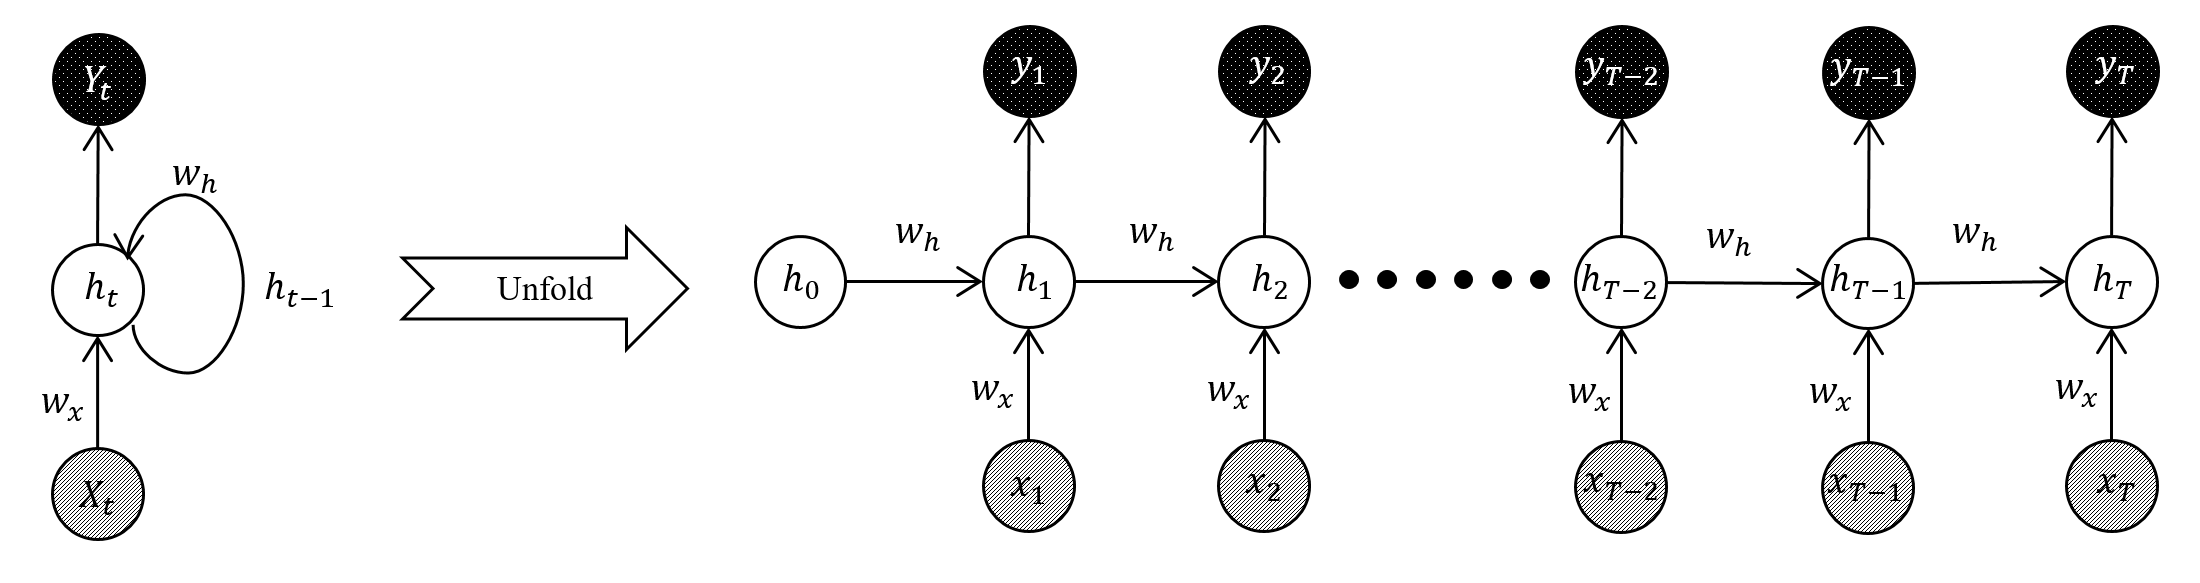
\includegraphics[width=1\textwidth]{rnn.PNG}
	\caption{Unfolding a RNN into a forward-feeding deep neural network.}
	\label{fig:rnn}
\end{figure}

\paragraph{Forward propagation} The first stage of the backpropagation algorithm calculates the network output using the current model weights. We can illustrate this using a typical Elman network with \(H\) neurons arranged in a single hidden layer, \(P\) input dimensions and \(K\) output dimensions. The output of the \(h\)\textsuperscript{th} hidden recurrent neuron at time \(y\) is denoted as \(h^t_h\). The weighted sum of all input dimensions at the current time step is added to the weighted sum of hidden activations at the previous step and a shared bias \eqref{forward_prop_weighted_sum}. The value is then activated through a non-linear activation function \eqref{forward_prop_activation}.

Forward propagation
\begin{subequations} 
	\begin{equation}
	\label{forward_prop_weighted_sum}
	x^h_t=b^h+\sum_{p=1}^{P}w_{p,h}x^p_t+\sum_{h^\prime=1}^{H}w_{h^\prime,h}h_{t-1}^{h^\prime}
	\end{equation}
	\begin{equation}
	\label{forward_prop_activation}
	h_t^h=f(x_t^h)
	\end{equation}
\label{forward_prop}
\end{subequations}

The activated output \(h^h_t\) is recursively calculated for each neuron by incrementing time step \(t=1,2,3,...,T\). Once all hidden outputs have been calculated for all the \(H\) hidden neurons, the network output \(\hat{Y}_t^k\) of the \(k\)\textsuperscript{th} dimension at time \(t\) is simply the weighted sum of all hidden activations at the same time step for a regression problem. Using the forward propagation algorithm, the network output can be calculated at every time step.


\paragraph{Weight Update} 
The model's output is compared with the expected output (i.e. training labels) in order to calculate the loss \(\mathcal{L}\) with respect to the current set of parameters. The loss function  is a hyperparameter of the ANN. For regression problems, commonly-used loss functions include mean-squared error (MSE), mean absolute percentage error (MAPE) and mean absolute error (MAE).

Network output and loss function
\begin{subequations} 
	\begin{equation}
	\label{dense_output}
	\hat{Y}^k_t=\sum_{h\prime=1}^{H}w_{h^\prime,k}h^{h\prime}_t
	\end{equation}
	\begin{equation}
	\label{loss_function}
	\mathcal{L}_w=f(\hat{Y}^t,T^t)
	\end{equation}
\end{subequations}

In this stage, the algorithm tries to improve the loss function by modifying the weights. To achieve this, partial derivative is applied to the loss function to find out the gradients with respect to each weight. In RNNs, this step is very similar to regular weight update in simple ANNs. The only exception is that the gradient depends on both the output as well as the information inherited from previous time step. For example, the gradient of the \(h\)\textsuperscript{th} hidden neuron is given by the following formulae where all of the \(K\) outputs and \(H\) hidden neurons are involved.

The gradient is recursively calculated backwards, starting from \(t=T\) until it reaches the beginning of the sequence. The gradient with respect to each of the weight is calculated as the sum of the whole sequence over time. The weights are then updated iteratively and the backpropagation process starts again.

Network output and loss function
\begin{subequations} 
	\begin{equation}
	\label{differentiation}	
	\delta^h_t=\frac{\partial{L}}{\partial h^h_t}	
	\end{equation}
	\begin{equation}
	\label{weight_update}
	\delta^h_t=f(h^h_t)\Bigg(\sum_{k=1}^{K}\delta_k^tw_{h,k}+\sum_{h^\prime=1}^{H}\delta_{h^\prime}^{t+1}w_{h,h^\prime}\Bigg)
	\end{equation}
\end{subequations}


\subsubsection{Unstable Gradient}

Common activation functions such as sigmoid and hyperbolic tangent squeeze the input space into a very small and fixed range. If the network is very deep (e.g. an unrolled RNN with long sequence), the activation of earlier layers would be mapped to an even smaller range in later layers. This means that large changes in earlier layers would cause insignificant changes in later layers. As a result, the gradient in earlier layers would be unavoidably small. Recalling the core principle of backpropagation, this would result in very slow learning in layers with weak gradients. This leads to the vanishing gradient problem which haunts deep ANNs as well as RNNs with long training sequence \cite{hochreiter1991, hochreiter2001}.

The opposite of vanishing gradient is exploding gradient. It happens in a deep network when the gradients are large, as the multiple of many positive values yields a very large number. In some extreme cases, the weight update step can fail as the new weights exceed the precision range. Such problem can be mitigated by weight clipping \cite{pascanu2012}.

Unstable gradients can be avoided by using alternative activation functions which do not forcibly squeeze input space into a narrow range. For instance, rectifier activation (e.g. ReLU) can provide robust gradient over any positive range. Another way to avoid the unstable gradient problem is to use different recurrent neuron structures which will be discussed in the next section.

\subsubsection{Long Short-Term Memory}

As simple RNNs suffer from unstable gradient problem, they are ineffective in learning long term dependencies. There has been previous attempts to address this problem by using non-gradient descent learning methods \cite{bengio1994}. Yet one of the most popular ways is to use a neuron structure called long short-term memory (LSTM), originally proposed by Hochreiter \& Schmidhuber \cite{hochreiter1997} and subsequently improved in later years \cite{gers2000, gers2003, graves2012}.

Like simple recurrent neuron, the LSTM block aims at learning pattern over time by carrying information from previous time steps. However, the LSTM block structure is much more complicated. There are multiple gates controlling the flow of information. Figure \ref{fig:lstm} adopted from Olah \cite{olah} illustrates the internal structures of a LSTM block:


\begin{figure}[H]
	\centering
	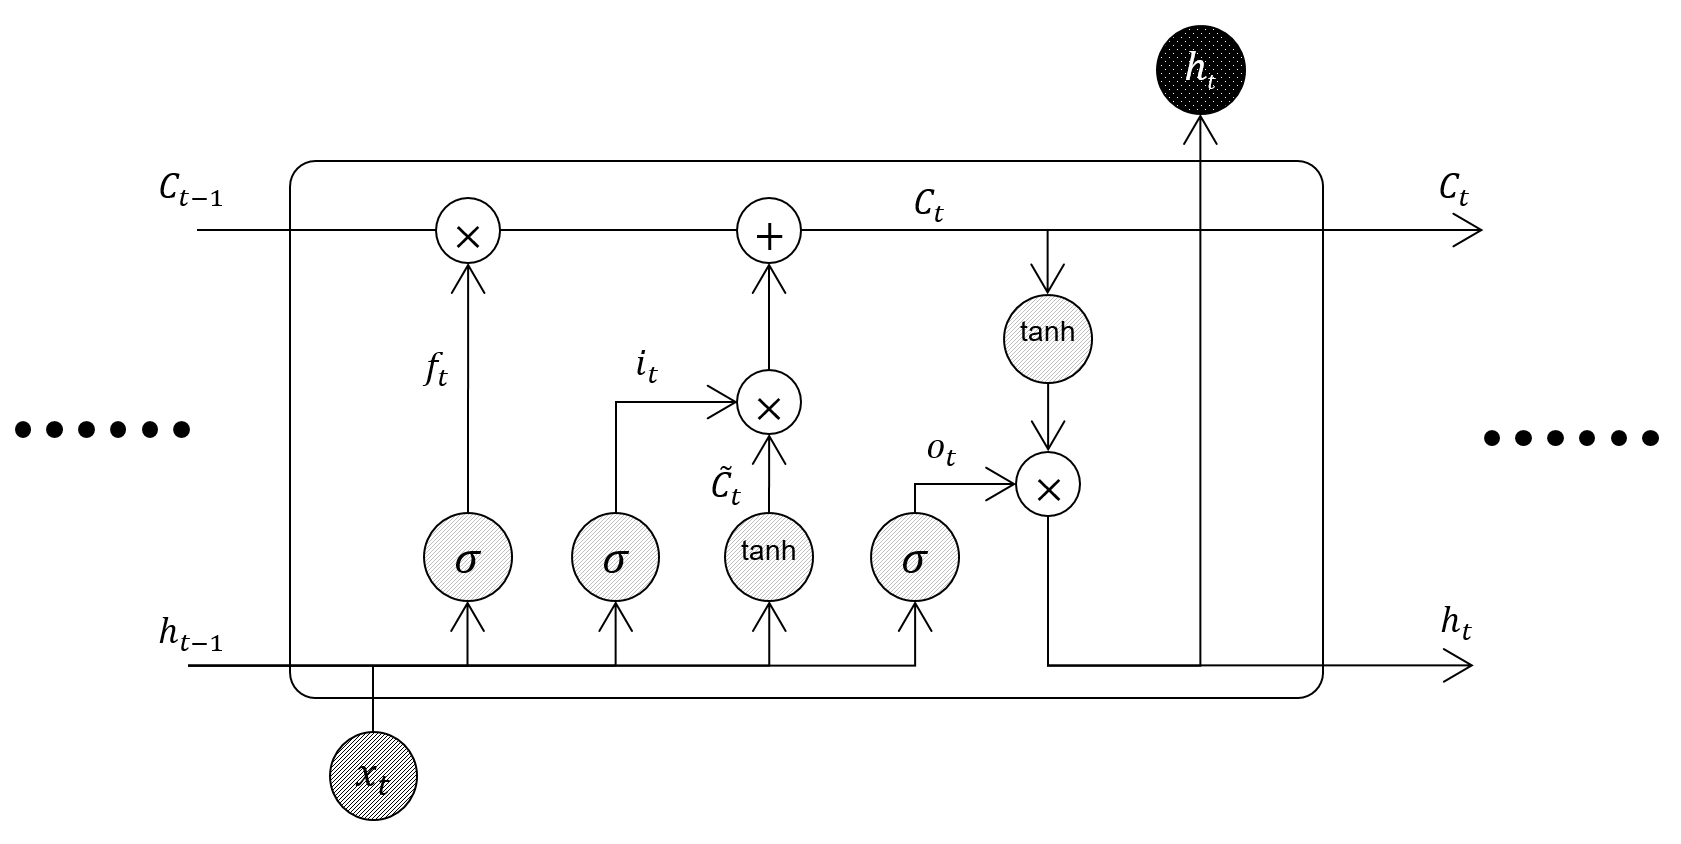
\includegraphics[width=1\textwidth]{lstm.PNG}
	\caption{Internal structure of a long short-term memory block.}
	\label{fig:lstm}
\end{figure}


Each LSTM block carries a hidden state denoted as \(C_t\) which holds the recurrent information. It is updated by identifying what needs to be forgotten and what needs to be remembered, given the current input \(x_t\) and the activation at previous step \(h_{t-1}\).

The forget gate on the leftmost side contains a sigmoid function. It reads the information and computes a real value \((0,1)\) which indicates the portion of information to forget (i.e. closer to \(0\)) or to retain (i.e. closer to \(1\)) \eqref{lstm_forget}.

Similar to the forget gate, another sigmoid function called the input gate determines the amount of information to remember at the current time step which is denoted as \(i_t\). The input gate is also computed using the current input \(x_t\) and previous step’s output \(h_{t-1}\) but with a different weight vector \eqref{lstm_input1}. Then a hyperbolic tangent function yields a real value \((-1,1)\) to decide how much to update \eqref{lstm_input2}.

Lastly, the new hidden state \(C_t\) can be updated by multiplying the forget gate value \(f_t\) with the previous hidden state of the neuron \(C_{t-1}\), then adding input gate value \(i_t\) scaled with the hyperbolic tangent function output \(\tilde{C}_t\) \eqref{lstm_update_hidden}.

Simultaneously, the output gate is computed with sigmoid function using the same parameters \(x_t\) and \(h_{t-1}\) \eqref{lstm_output1}. Meanwhile the updated hidden state \(C_t\) goes through a hyperbolic tangent function to decide the portion of information to output. These two parts multiply together to form the recurrent output \(h_t\) of the current time step \eqref{lstm_output2}.

\begin{subequations} 
	
	Forget gate
	\begin{equation}
	\label{lstm_forget}
	f_t=\sigma(W_f[h_{t-1},x_t]+b_f)
	\end{equation}
	
	Input gate
	\begin{equation}
	\label{lstm_input1}
	i_t=\sigma(W_i[h_{t-1},x_t]+b_i)
	\end{equation}
	
	\begin{equation}
	\label{lstm_input2}
	\tilde{C}_t=\tanh (W_c[h_{t-1},x_t]+b_C)
	\end{equation}
	
	Update hidden state
	\begin{equation}
	\label{lstm_update_hidden}
	C_t=f_t\times C_{t-1}+i_t\times\tilde{C}_t
	\end{equation}
	
	
	Output gate
	\begin{equation}
	\label{lstm_output1}
	O_t=\sigma(W_o[h_{t-1},x_t]+b_o)
	\end{equation}
	
	\begin{equation}
	\label{lstm_output2}
	h_t=O_t\times\tanh C_t
	\end{equation}
\end{subequations}


As the LSTM block uses various gates to control information flow, recurrent information can be carried over to further down the time line as it is protected from being overwritten. For example, the recurrent hidden state \(C_t\) cannot be overwritten by the current input \(x_t\) if the input gate is not open (i.e. the \(\tilde{C}_t\) value close to zero). This allows the LSTM block to avoid unstable gradient and therefore able to learn long-term temporal dependency over multiple steps.


\subsubsection{Regularisation}

ANN’s non-linear capability implies that it is a very flexible modelling technique which is prone to overfitting. To overcome this problem, a randomly selected fraction of neurons can be temporarily removed during training \cite{srivastava2014}. This technique called dropout forces the neurons to work with the remaining network more robustly and hence prevents overfitting. It soon becomes a common technique for ANN regularisation.

In an RNN setting, dropout can amplify error when applied to recurrent connections. Zaremba et al. \cite{zaremba2014} suggested that dropout should only be applied non-recurrent connections (e.g. between hidden layers). This helps the recurrent neurons to retain memory through time while still allowing the non-recurrent connections to benefit from regularisation.

\begin{figure}[H]
	\centering
	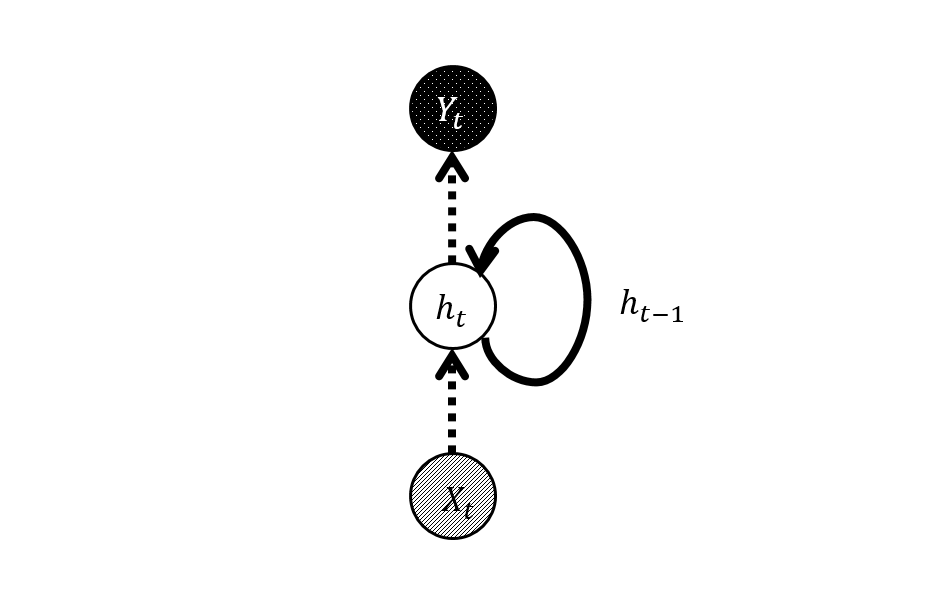
\includegraphics[width=0.5\textwidth]{dropout.PNG}
	\caption{Application of dropout in RNN. Dotted arrows indicate non-recurrent connections where dropout is applied. Solid arrow indicates recurrent connection without dropout.}
	\label{fig:dropout}
\end{figure}

\subsection{Sequence-to-Sequence Model}

Sequence-to-sequence (seq2seq) is a type of RNN model. It has an encoder-decoder structure where both are made up of multi-layered recurrent neurons. The purpose of seq2seq model is to provide end-to-end mapping between an ordered multidimensional input sequence and its matching output sequence. The model has been widely used to solve machine translation tasks where words in a sentence are considered as input/output vector sequences\cite{sutskever2014, cho2014}. The model can also generate sentences which enabled meaningful human-machine conversation \cite{vinyals2015}. Modified seq2seq model can perform complex tasks such as image and video captioning as well \cite{venugopalan2014, vinyals2014}. Yet, the power of seq2seq does not limit to the aforementioned areas. It is a generic modelling technique for handling any sequential input and output data.

Eventually this brought us back to the original signal analysis problem. As we discussed in earlier sections, a large-scale industrial process with sensor data collected at various locations can be treated as a multidimensional entity changing through time. This implies that seq2seq model can be extended to the area of signal analysis in order to leverage recurrent neuron’s power to understand complex and time-dependent relationship.

Figure \ref{fig:seq2seq} below graphically illustrates a seq2seq model. The RNN-based encoder reads an input sequence and summarises all information into a fixed-length vector at the context layer. The decoder then reads the vector and predicts the target sequence.

\begin{figure}[H]
	\centering
	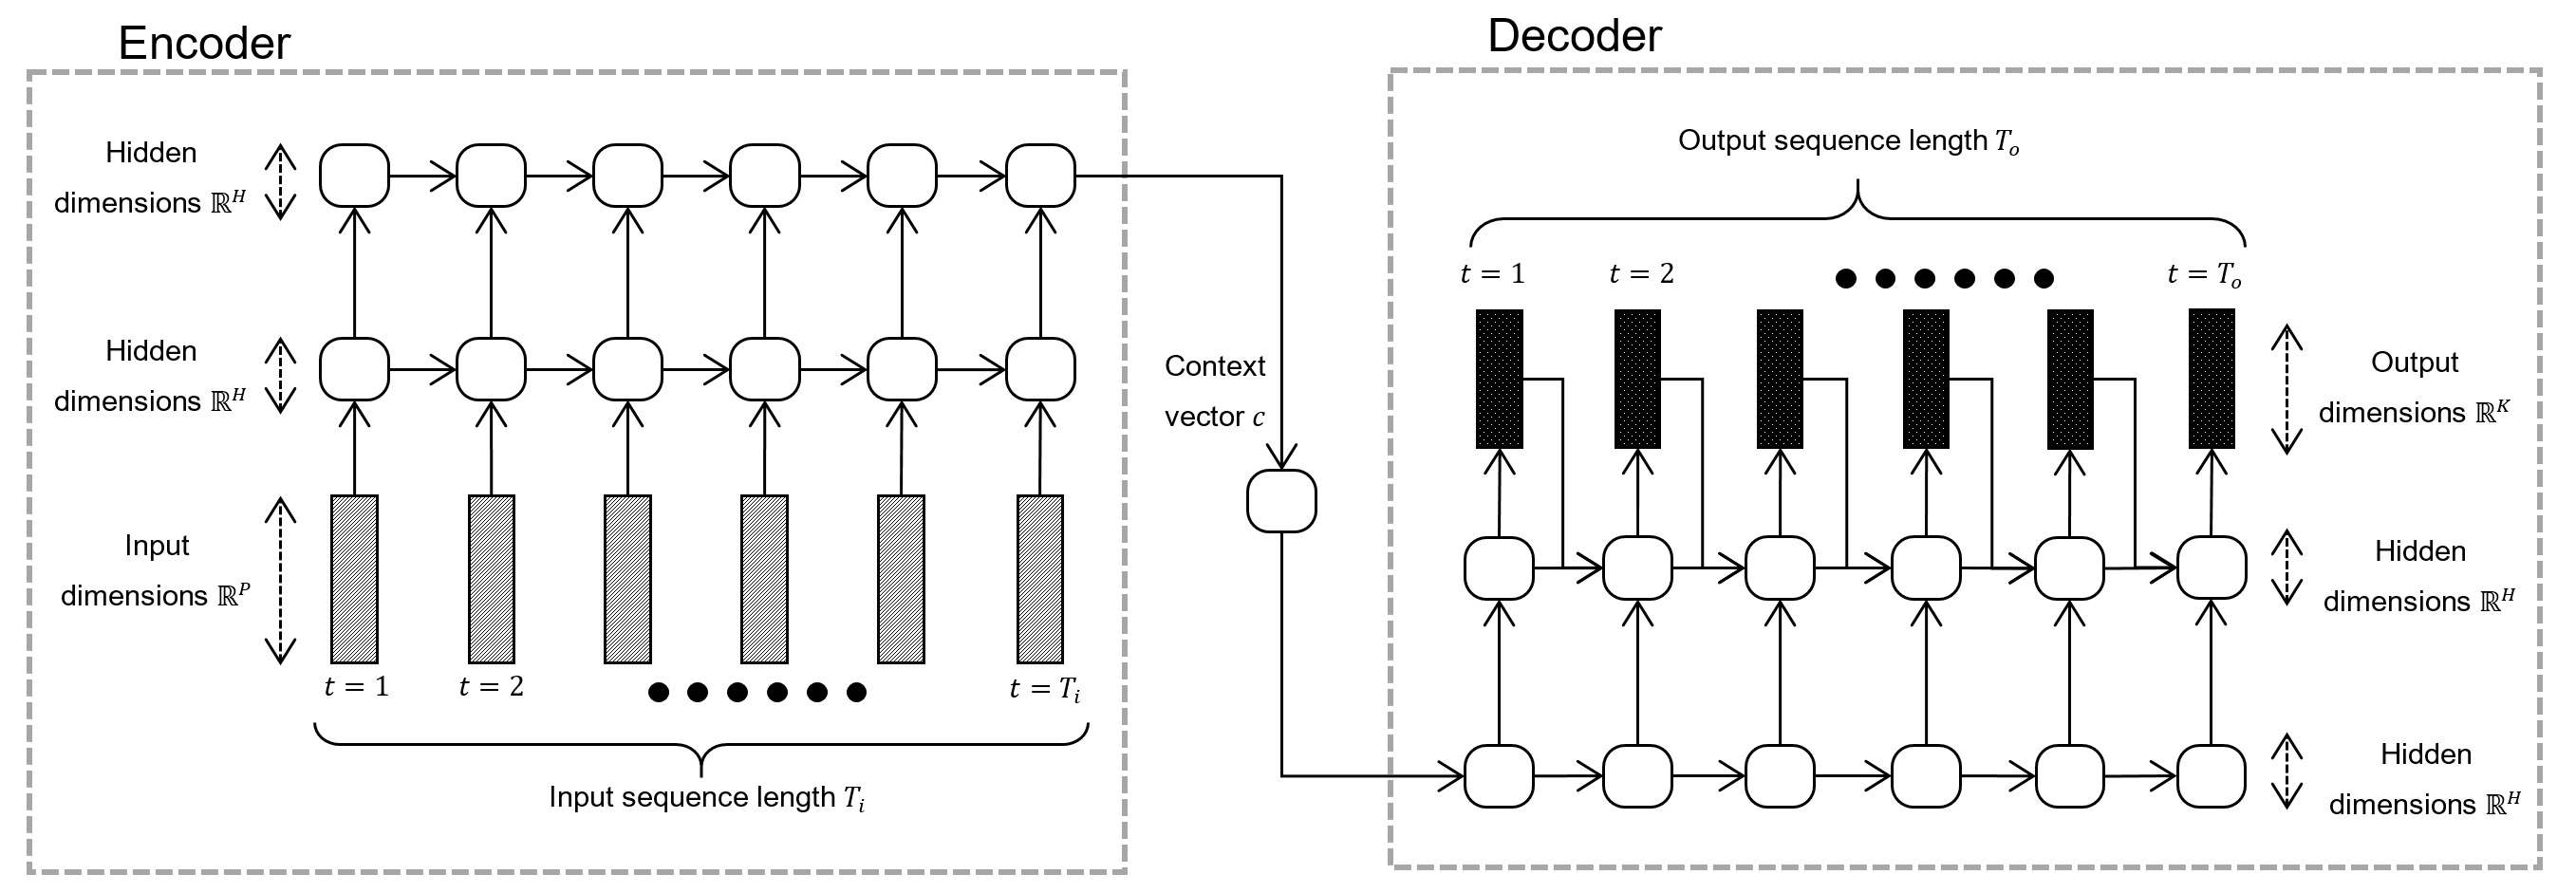
\includegraphics[width=1\textwidth]{seq2seq.PNG}
	\caption{Seq2seq model with multiple hidden recurrent layers. Both the encoder and decoder are made up of multilayered RNN. Arrows indicate the direction of information flow.}
	\label{fig:seq2seq}
\end{figure}

\subsubsection{Encoding} The role of the recurrent encoder is to project the multidimensional input sequence into a fixed-length hidden context vector \(c\). It reads the input vector of \(\mathbb{R}^P\) dimensions sequentially from \(t=1,2,3,...,T_i\) where the input sequence contains \(T_i\) time steps. The hidden state of the RNN made up of \(\mathbb{R}^H\) dimensions updates at every time step based on the current input and hidden state inherited from previous step \eqref{seq2seq_encoder1}. The input sequence length \(T_i\) is fixed during training and prediction as well. This would allow the model to capture temporal patterns at maximum length \(T_i\).

The dimension of the input sequence is also fixed for training and prediction. In order to leverage the RNN encoder’s power to learn complex patterns over time, the input dimension of the proposed model is made up of all available sensors. Recurrent neurons arranged in multiple layers are capable of learning complex time-dependent behaviours. In most seq2seq models, LSTM neurons are usually used. Cho et al. \cite{cho2014} suggested using gated recurrent neuron (GRU) which may improve model training efficiency. Once the recurrent encoder read all the input information, the sequence is summarised in a context vector \(c\) which is a  fixed-length multidimensional vector representation \(\mathbb{R}^H\) \eqref{seq2seq_encoder2}.

The function of the encoder structure is to maps a time-ordered sequence of multidimensional vector into a fixed-length vector representation \eqref{seq2seq_encoder3}. In this way, the RNN encoder achieved a compression ratio of \( \frac{T_i*P}{H} \). The compression ratio should be high enough in order to provide a choke point, so that the encoder can learn useful knowledge. The model may risk learning a useless identify function if the compression ratio is too low (e.g. hidden dimension \(H\) is too large) \cite{goodfellow}.

As the seq2seq network is trained end-to-end, the context vector is a representation of the input sequence conditioned on corresponding output sequence. This implies that the context vector can provide useful knowledge in relation to the input-output sequence pair, such information can be analysed in order to generate meaningful diagnostic measurements which we will discuss later.

\begin{subequations} 
	
	Update hidden state of encoder
	\begin{equation}
	\label{seq2seq_encoder1}
	h_t = f(h_{t-1}, x_t), t=1,2,3,...,T_i
	\end{equation}
	
	Output context vector
	\begin{equation}
	\label{seq2seq_encoder2}
	c = f(h_{T_i})
	\end{equation}
	
	Encoder function
	\begin{equation}
	\label{seq2seq_encoder3}
	f_{encoder} : \{ \mathbb{R}_t^P:t \in [1,T_i] \} \rightarrow c
	\end{equation}
	
\end{subequations}

\subsubsection{Decoding}
The decoder is a recurrent network which converts the context vector \(c\) into the sequence of output vector. To exemplify this, the decoder starts by reading the context vector \(c\) at \(t=1\) \eqref{seq2seq_decoder1}. It then decodes the context information through the recurrent multilayer structure and outputs the vector \(y_1\) at the first decoder time step which maps back to \(\hat{Y}_1\) in the final layer. Afterwards, the decoder's hidden state is passed on to the next time step and the new state is computed based on the previous state \(h_{t-1}\) as well as the previous vector output \(y_{t-1}\) \eqref{seq2seq_decoder2}. The RNN decoder carries on making predictions at each output step until it reaches the total length of the output sequence length \(T_o\). In essence, the decoder decompresses the information stored in the context vector into the output multidimensional sequence \eqref{seq2seq_decoder3}.

\begin{subequations} 
	
	Initiates decoder
	\begin{equation}
	\label{seq2seq_decoder1}
	h_1=f(c)
	\end{equation}
	
	Update hidden state of decoder
	\begin{equation}
	\label{seq2seq_decoder2}
	h_t = f(h_{t-1}, y_{t-1}), t=2,3,4,...,T_o
	\end{equation}
	
	Decoder function
	\begin{equation}
	\label{seq2seq_decoder3}
	f_{decoder} :  c \rightarrow \{ \mathbb{R}_t^K:t \in [1,T_o] \}
	\end{equation}
	
\end{subequations}

\subsubsection{Recurrent Autoencoder}

Recurrent autoencoder is a specific kind of RNN which maps input data back into itself through a neural encoder-decoder structure. The encoder structure compresses multidimensional input data in a vector representation, while the decoder structure then receives this information and reconstructs the original data. Seq2seq model can easily be converted into an autoencoder setting with recurrent properties. It can be achieved by fixing input sequence length \(T_i\) and output sequence length \(T_o\) to be identical, or we can simply denote the length as \(T\).

\paragraph{Dimensionality Relaxation}

Recalling one of the fundamental characteristics of an autoencoder is the ability to map input data back into itself via a context vector representation. This criterion can be slightly relaxed such that output dimension \(K\) is smaller than input dimension \(P\), which means the output \(\{\mathbb{R}_t^K:t\in [1,T] \}\) is a subset of input \(\{\mathbb{R}_t^P:t\in [1,T] \}\) \eqref{seq2seq_autoencoder_relax_encoder}. As a result, the encoder receives a high dimensional input but the corresponding decoder is only required decompress a subset of the original dimensions in the output sequence. End-to-end training of the relaxed seq2seq autoencoder suggests that the context vector would summarise the input sequence while still being conditioned on the output sequence.

Seq2seq autoencoder with output dimensionality relaxation
\begin{equation}
\label{seq2seq_autoencoder_relax_encoder}
\begin{cases} 
f_{encoder} : \{  \mathbb{R}_t^P:t \in [1, T] \} \rightarrow c \\
f_{decoder} : c \rightarrow \{  \mathbb{R}_t^K:t \in [1, T] \} \\
\end{cases} K \leqslant P
\end{equation}

Having a subset of dimensions in the outputs sequence has a significance for practical application of the algorithm. In the industrial process use case, all streams of sensor readings are included in the input dimension while only part of the selected sensors would be included in the output dimensions. This means the entire process state is visible to the encoder RNN, thus enabling it to learn complex patterns efficiently.

More importantly, the context vector is conditional on the selected sensors as defined in the output dimensions. It only activates if the decoder captures patterns in the set of selected sensors in the output sequence. Similar sensor patterns across different samples would result in very similar activation in the hidden context vector as they are located in the close vicinity of each other. Contrarily, abnormal sensor patterns would lead to activation in relatively distant space which effectively provide means to distinguish irregular pattern and usual behaviour.

Given that the context vector is a compressed and timeless summary of complex pattern in the input-output sequences pair, it can be used as diagnostic measurement for the process state while being conditioned on the key sensors. Following this logic, several seq2seq autoencoder models can be trained using different output dimensions in order to capture different patterns across different sensor sets.

\paragraph{Consecutive Sampling}

As the length of input and output sequences are fixed as \(T\) in the seq2seq autoencoder model, the time series input drawn from the subset sequence must have same length too. To generate training samples from a subset of length \(T^\prime\) where \(T^\prime > T\), we can begin at \(t=1\) and draw a sample of length \(T\). This process continues recursively by shifting one time step until it reaches the end of the subset sequence. It directly enables online training and prediction which is essential for time-critical applications like sensor data processing. For a subset sequence of length \(T\), this method allows \(T^\prime - T\) samples to be generated.


\begin{algorithm}[H]
	\label{consecutive_sampling}
	\caption{Consecutive Sampling}
	
	\SetKwInOut{Input}{Input}
	\Input{Sample sequence length \(T\)}
	\Input{Subset sequence length \(T^\prime\)}
	
	\(i\leftarrow 0\) \;
		\While{\(i \leqslant i+T \) }{
			Generate sample sequence \( (i, i+T  ] \) from the subset sequence\;
			\(i\leftarrow i+1\)\;
		}
\end{algorithm}


\begin{figure}[H]
	\centering
	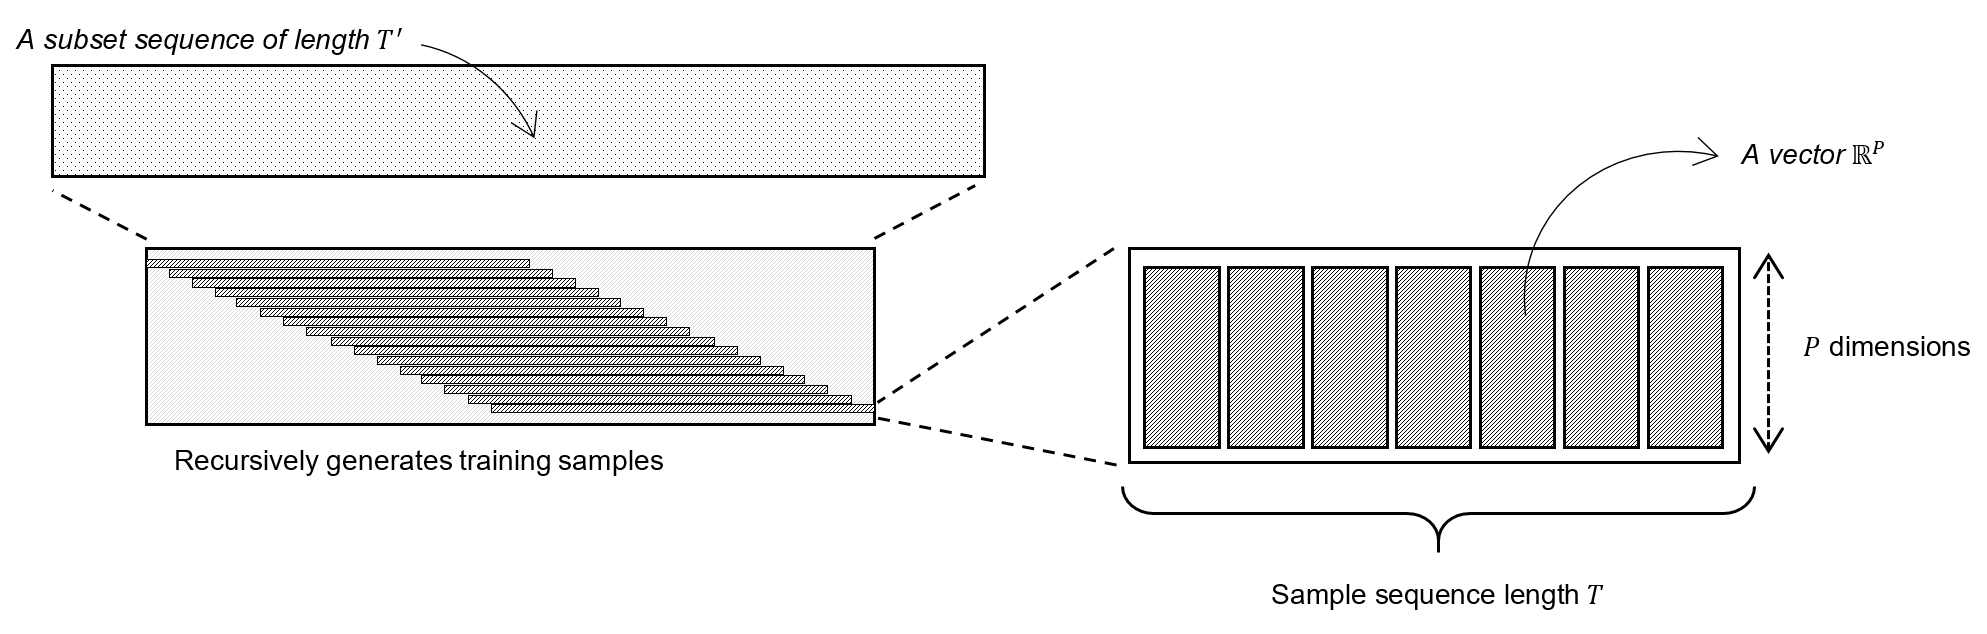
\includegraphics[width=1\textwidth]{consecutive_sampling.PNG}
	\caption{Drawing consecutive training sample sequences recursively from a subset}
	\label{fig:consecutive_sampling}
\end{figure}

\paragraph{Encoder Output} 

Given that sample sequences are recursively generated by shifting one time step, successive sequences are highly correlated with each other. This means that when they are fed through the encoder structure, the context activation \(c\) would also be highly correlated. As a result, consecutive context vectors can join up to form a smooth path in high dimensional space. In theory, they can be visualised in lower dimensions via dimensionality reduction techniques such as principal component analysis (PCA).

As we have discussed previously, the fixed-length context representations summarise information in the input sequence. Context vectors in the same neighbourhood have similar activation therefore can be considered belonging to a similar underlying state. Contrarily, context vectors located in different neighbourhoods have different underlying state. In light of this, clustering techniques can be applied to the context vectors in the training set in order to group similar sequences together. Each context vector can be assigned to a cluster \(C_j\) where \(J\) is the total number of clusters \eqref{clustering_context_vector}. 

Assigning cluster to context vector
\begin{equation}
\label{clustering_context_vector}
c \rightarrow C_j , j\in \{1,2,3,...,J\}
\end{equation}

Once all the context vectors are labelled with their corresponding clusters, supervised classification algorithms can be used to learn the relationship between them using the training set. For instance, support vector machine (SVM) classifier with \(J\) classes can be used. The trained classifier can then be applied to the context vectors in the held-out validation set in order to assign clusters. The process state can be considered changed when successive context vectors move from one neighbourhood to another (e.g. the context vector substantially drifting away from current neighbourhood leading to different cluster assignment).

\newpage

\section{Results}
Various seq2seq autoencoder models were trained with different hyperparameters. The choice of hyperparameters has vast implications on the properties of the model which we will discuss further alongside empirical evidence.

\subsection{Setup}

The raw sensor dataset was recorded at highly granular level but at irregular interval. It was transformed into regularly-spaced time series using tumbling window approach with standard window size \(W=600\) seconds (\(5\) minutes). Elements within each window were aggregated by taking the simple arithmetic average of all members. Training samples were drawn from the sample consecutively with sequence length \(T=36\) (\(3\) hours). The model has input dimensions \(P=158\) and output dimensions \(K=6\) where the selected set of sensors in the output are key performance indicators of the two-stage compression train.

The dataset was divided into two parts, where the first \(70\) percent of the data belongs to the training set and the remaining belongs to the validation set. In total, there are \(2543\) sequences in the whole dataset.

Both the training and validation sets were standardised into \(z\)-scores. The mean of each dimension \(\bar{x}_p\) is removed and the difference from mean is divided by the standard deviation of the dimension \(\sigma_p\) \eqref{zscore}. It makes sure that the all dimensions contain zero-centred values which facilitates gradient-based training.

Standardising dataset using \(z\)-score
\begin{equation}
\label{zscore}
z_p=\frac{x_p-\bar{x}_p}{\sigma_p}
\end{equation}

All models were trained at 32-bit precision on a single Nvidia Quadro P5000 device.

\subsection{Training Models}

We have conducted several experiments on various hyperparameters and they were found to have drastically different effects on the model's properties. All models were trained for \(5000\) epochs and the gradient was clipped at \(0.3\) to avoid the exploding gradient problem.

\subsubsection{Batch Size}

We have assessed the effects of different batch sizes using Minibatch Gradient Descent optimiser. It uses one batch of training samples to perform gradient evaluation. This means when the batch size \(B\) is closer to sample's total size \(N\) its behaviour would resemble classic batch gradient descent. Alternatively, when \(B\) gets smaller or even closer to \(1\) then it would behave like SGD optimiser.

Varying batch size \(B\) has subtle effects on the optimiser's properties as seen in figure \ref{fig:minibatch_batch_size}. It is clearly illustrated that the loss function converges a lot quicker when \(B\) is small. This is simply because more gradient updates can be packed in a single epoch.

\begin{figure}[H]
	\centering
	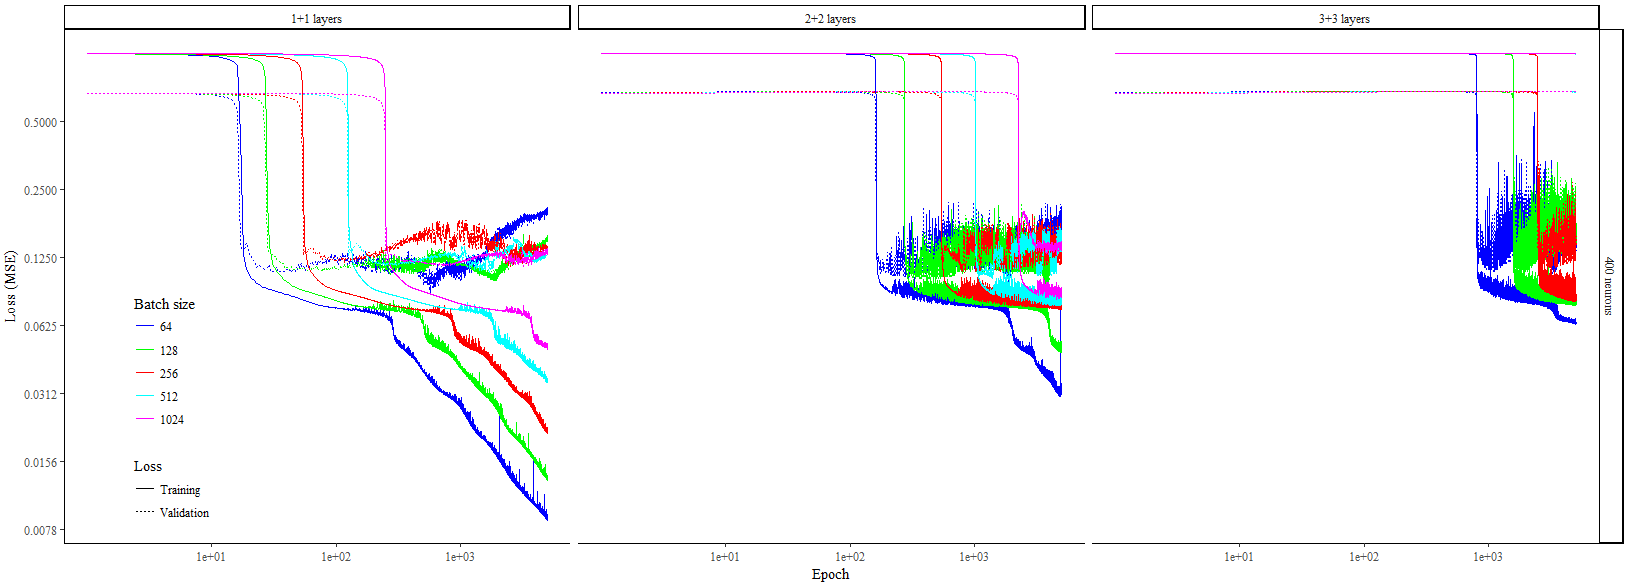
\includegraphics[width=1\textwidth]{minibatch_batch_size.PNG}
	\caption{Several sets of auutoencoder models were trained using minibatch gradient descent optimiser with different batch sizes. They contain \(1+1\) layers, \(2+2\) layers and \(3+3\) layers in the encoder-decoder structures respectively. All hidden layers contain \(400\) neurons. Both \(x\)- and  \(y\)-axes are in logarithmic scale.}
	\label{fig:minibatch_batch_size}
\end{figure}

In theory, the variance of gradient update also becomes higher when the batch size is small. Volatile gradient update encourages the parameters to improve by jumping towards different directions. Contrarily, large batch size leads to consistent gradient update thus discourages parameter jumping. The effect is only very marginal as seen in the \(1+1\) layer scenario, where the validation MSE for smaller batch size is slightly lower that the others.

As the number of hidden layers increases, Minibatch Gradient Descent becomes much less efficient regardless of the batch size. The training and validation losses of \(3+3\) layers models remain fairly stagnant comparing with shallower models. Only smaller \(B\) values were able to bring marginal improvements in deep models.

\subsubsection{Learning Rate}

The learning rate \(\mu\) is a crucial hyperparameter of the optimiser which determines the size of gradient update. On one side, small learning rate allows tiny steps to be made which encourages better convergence at minima. On the other side, large learning rate allows rapid learning but it is vulnerable to divergence. Figure \ref{fig:learning_rate} below shows the effects of different learning rates on the training and validation MSEs.

\begin{figure}[H]
	\centering
	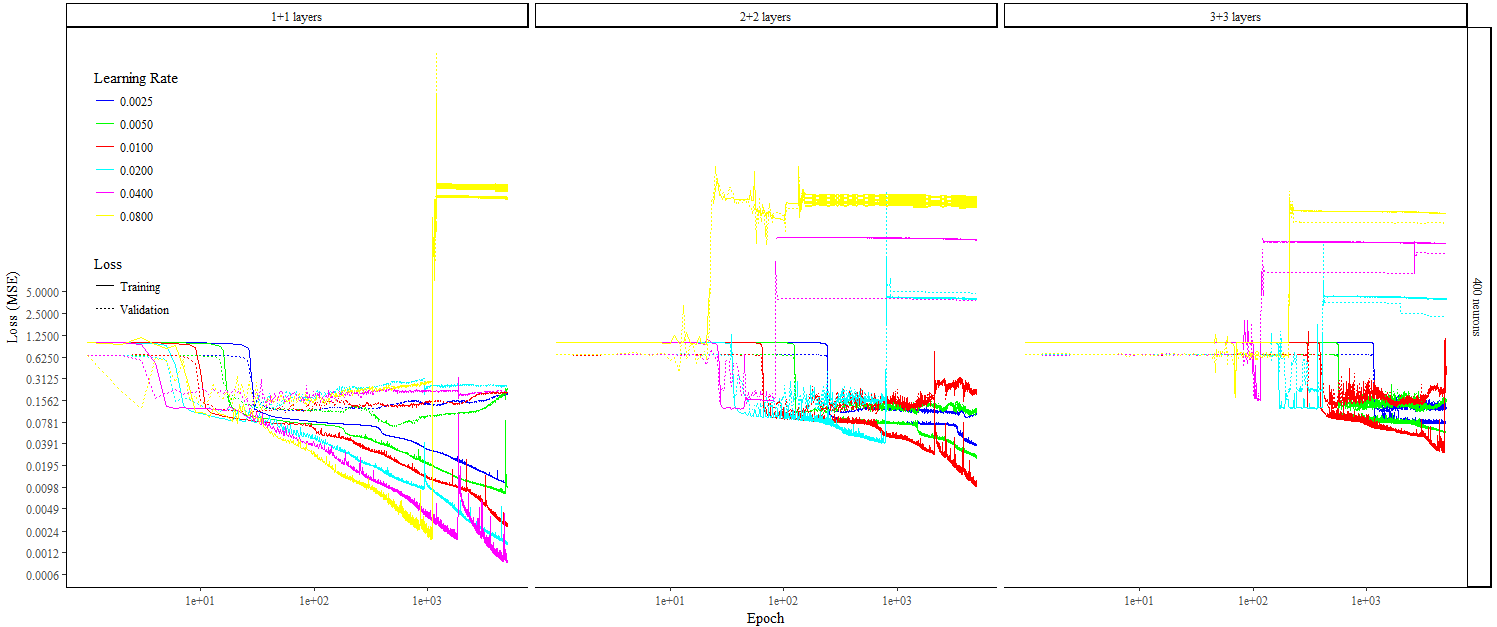
\includegraphics[width=1\textwidth]{learning_rate.PNG}
	\caption{Training and validation losses of minibatch gradient descent optimisers. Three sets of models containing different number of hidden layers were trained. All models have \(400)\) neurons in each hidden layer.}
	\label{fig:learning_rate}
\end{figure}

As shown by the autoencoder model with \(1+1\) layer structure in figure \ref{fig:learning_rate}, the model is able to converge earlier at a higher learning rate. However, the model becomes prone to overshooting with high learning rate as suggested by the \(\mu=0.08\) scenario. Both the training and validation losses experienced a significant increase which indicates divergence. This phenomenon becomes more evident when the model has deeper structure. The models with \(2+2\) and \(3+3\) layers structures shown significant divergence at much earlier epochs with even smaller learning rates. This highlights the challenges we faced when training deep and complexed RNN structures. It eventually suggests more advanced optimisers should be used.

\subsubsection{Advanced Optimisers}

We have added various optional improvements to the minibatch gradient descent optimiser and tested alongside other advanced optimisers. Again, three sets of comparablemodels were ran with different optimisers. All of them were executed with the default hyperparameters as recommended in their original publications which are outlined in the appendix.

\begin{figure}[H]
	\centering
	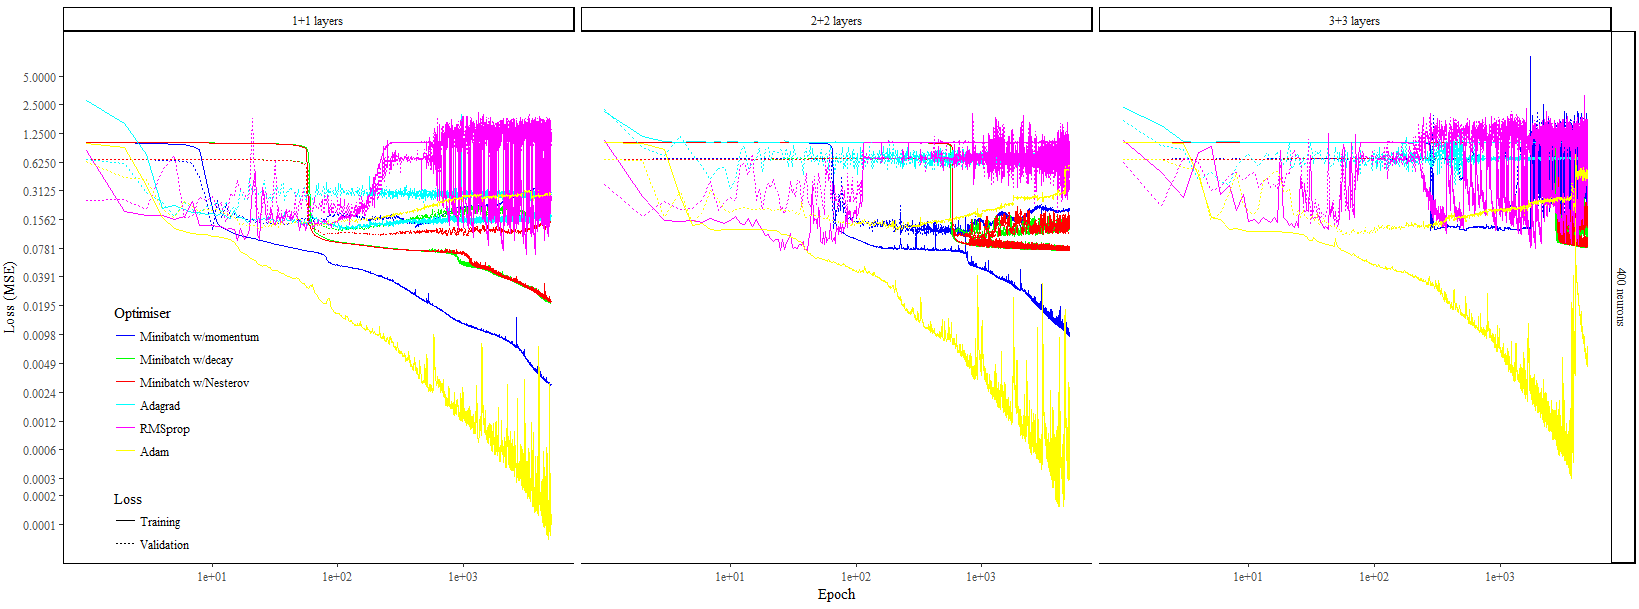
\includegraphics[width=1\textwidth]{optimisers.PNG}
	\caption{Training and validation losses of various optimisers. All models were trained with same batch size \(B=256\).}
	\label{fig:optimisers}
\end{figure}

In figure \ref{fig:optimisers}, different optimisers showed contrasting results. Minibatch gradient descent optimisers (momentum, decay and Nesterov momentum) managed to improve the training and validation losses of shallower \(1+1\) layer models. However, the training speed decreased dramatically when the model grows deeper with much of the earlier epochs staying stagnant.

Contrastingly, optimisers with adaptive learning rates such as Adagrad, RMSprop and Adam were able to deliver improvements at much earlier epochs for both shallow and deep models. This suggests that adapting the learning rate to each model parameter helps aids training models with large parameter space. Yet, Adagrad suffers from slow learning in later epochs as both training and validation MSEs flat out. This is caused by diminished learning rate as it is divided by a cumulative term which grows as training epoch proceeds.

Nevertheless, RMSprop shows lower losses across all models but suffers from divergence at later epochs. This suggests that the adaptive learning rates were still too high as the parameters were approaching minima positions, which eventually led to overshooting. This can be resolved by reducing the \(\rho\) value which allows the learning rate to adapt to more recent gradients. 

Among all optimisers tested, Adam was the only one which demonstrates outstanding effectiveness at training both shallow and deep models without causing divergence or slow learning. The training MSEs of Adam decrease continuously as epochs increase. The corresponding validation MSEs show gradual decrease simultaneously, followed by moderate increase without showing signs of parameter divergence. This shows that even with default configuration, Adam is a suitable optimiser for a wide range of models.

\subsubsection{Topology}

The processing power of the network is primarily determined by the topology. The following figure illustrates the MSE loss of several models trained with same hyperparameters except the number of neurons and the number of hidden layers. Notice that both the horizontal and vertical axes are in logarithmic scale for clearer visualisation.

\begin{figure}[H]
	\centering
	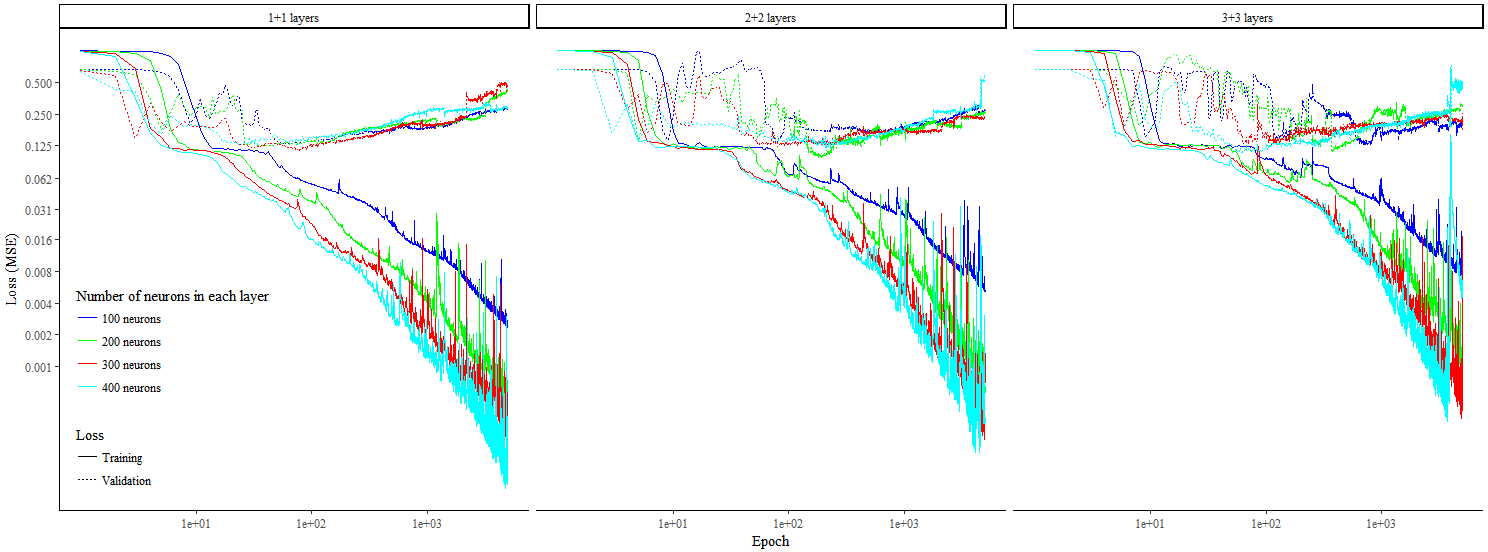
\includegraphics[width=1\textwidth]{loss_neuron_hidden.PNG}
	\caption{Effect of different number of neurons and hidden layers on training and validation loss. All models were trained with Adam optimiser (\(B=256\)).}
	\label{fig:loss_neuron_hidden}
\end{figure}

There are commonalities across different topological configurations. Firstly, the training losses of all models improve along successive plateaus and cliffs. Dauphin et al. \cite{dauphin} and Pascanu et al. \cite{pascanu2014} suggested that this is a problem of high dimensional data where the loss space is likely to be non-convex. In other words, the loss space is dominated by saddle points where minima exist in some dimensions but not in the others. The parameters experience lower gradients near the saddle point hence the loss function appears like a plateau. Once the optimiser learns a way to escape the saddle point, the training loss improves rapidly again.

Apart from this, the validation losses of all models share a common v-shape. It indicates that the knowledge learned by the models are generalisable to unseen data as the validation losses reach the minimum point. Gradual increase of the validation MSEs in later epochs suggest model overfitting. This means that the model is still learning on the training data but the knowledge acquired becomes less generalisable to the unseen validation data.

On the other side, changing the number of neurons while controlling the layer depth has effect on the MSE loss. Adding neurons provides additional non-linear computation as well as memory capacity to the models. The effect is consistent across all models as both training and validation MSEs decreases when more neurons were supplied.

Furthermore, altering the number of hidden layers while keeping the same number of neurons at each layer has various effects on the MSE loss too. For the training loss, shallow models show improvements much faster than deep models. An intuitive explanation for this phenomenon can be attributed to the shortened distance between input and output when the number of hidden layers is reduced. Although in theory deep models tend to outperform shallow models, they are much harder to train in reality. Error amplifies through deep structure which leads to inferior results, this suggests that regularisation is needed in order to train deep networks successfully.

\subsubsection{Dropout}

Regularisation is crucially important when it comes to training deep and complex model structures. We experimented the effects of different dropout rates on several models and their training and validation MSEs are illustrated in figure \ref{fig:dropout_chart} below.

\begin{figure}[H]
	\centering
	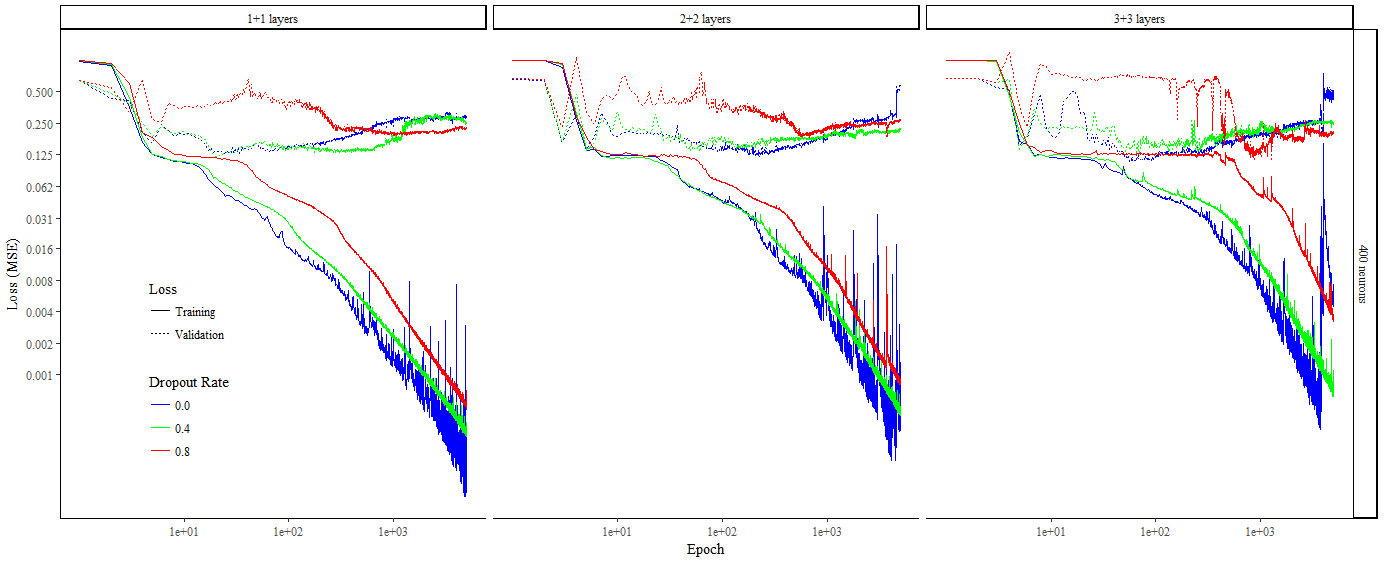
\includegraphics[width=1\textwidth]{dropout_chart.PNG}
	\caption{Chart showing the effects of various dropout rate.}
	\label{fig:dropout_chart}
\end{figure}

High dropout rate effectively masks substantially large part of the network which results in generally slower training. Despite this, it helps with suppressing the variance of model losses. The variance of training MSEs across all models are evidently lower with high dropout. 

Moreover, the models without dropout in both \(2+2\) and \(3+3\) layers scenarios show rapid training but eventually suffer from parameter divergence. High dropout was able to prevent this situation.

\subsubsection{Output Dimensions}

For an autoencoder model, the input and output dimensions are usually identical (i.e. \(K=P\)). However as we discussed earlier, the dimension of the output sequence can be relaxed such that \(K \leqslant P\). This allows the model to 

In the autoencoder model, the input sequence's dimensionality was represented by all the sensors of the entire system (\(P=158\)). The relaxed output dimensionality was set at \(K=6\) which includes a set of sensors reflecting key measurements of a specific aspect of the system process. We have experimented three scenarios where the first two have complete dimensionality \(P=158; K=158\) and \(P=6; K=6\) while the remaining scenario has relaxed dimensionality \(P=158; K=6\). The training and validation MSEs of these models are visualised in figure \ref{fig:output_dims} below.

\begin{figure}[H]
	\centering
	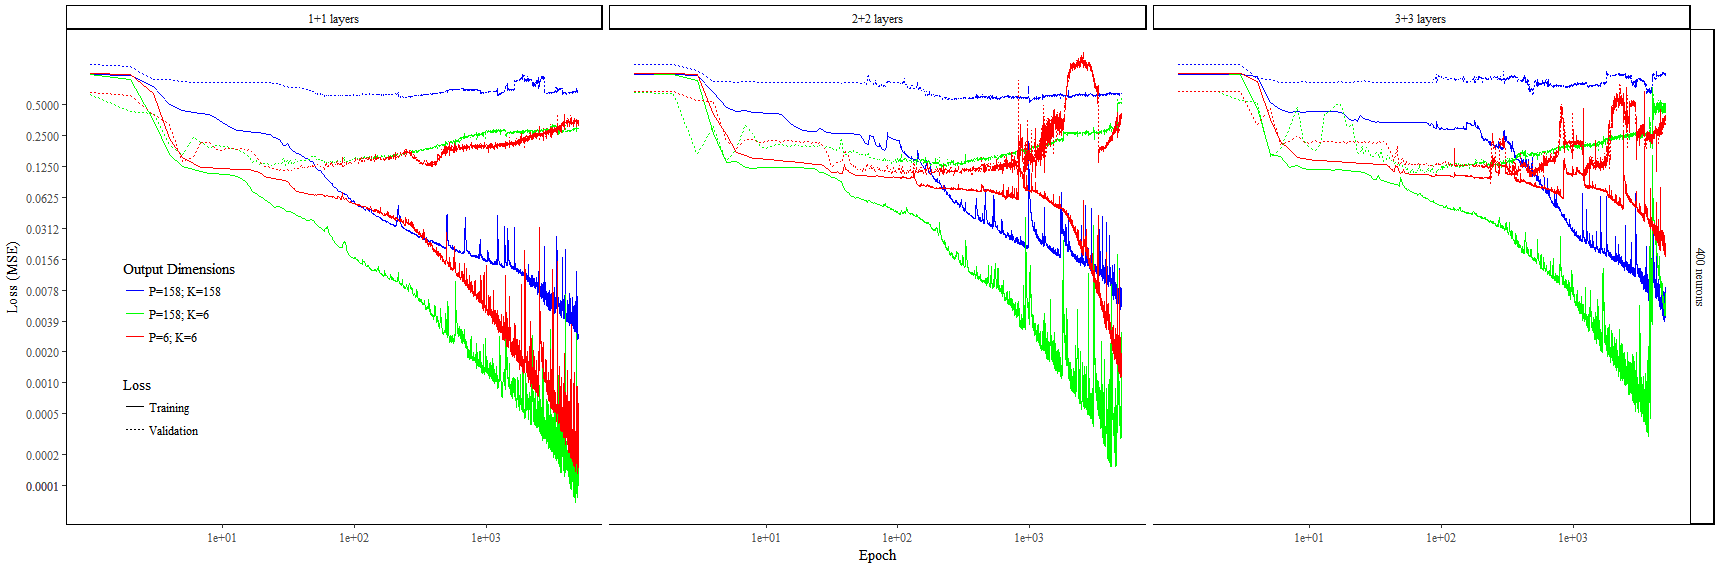
\includegraphics[width=1\textwidth]{output_dims.PNG}
	\caption{Effects of varying output dimensionality on the training and validation losses. Three sets of models were trained, each has different number of hidden layer in the encoder-decoder structure. All models have \(400\) neurons in each hidden layer. Models were trained with Adam optimiser at \(B=256\) with no dropout.}
	\label{fig:output_dims}
\end{figure}

The first model with complete dimensionality (\(P=158; K=158\)) has visibility of all sensors in both the encoder and decoder. The model show relatively slow improvement as they contain high dimensional data in both input and output sequences. This could be due to the lack of capacity in the RNN encoder-decoder structure to accommodate sequences at such high dimensionality.

For the complete dimensionality model with \(P=6; K=6\), the model has visibility to the selected dimensions only. The remaining dimensions (i.e. sensors of the entire system) were kept away from the encoder and decoder. This means that the autoencoder model is prohibited from learning any dependent behaviours among all the original dimensions. Besides, the model's capacity is too large for handling \(P=6; K=6\) thus leads to poor compression at the context layer. This led to poor generalisation as indicated by the high validation losses in deeper models.

Seq2seq autoencoder models with relaxed dimensionality demonstrate substantially lower training and validation MSEs across all scenarios. The third model has relaxed dimensionality with \(P=158; K=6\). This means that all dimensions are available in the encoder while the decoder only need to predict a subset of the input dimensions. This permits the autoencdoer model to learn dependency across all dimensions, leading to better and more consistent MSEs.

\subsubsection{Order Reversal}

Several models were trained with exactly the same hyperparameters with the exception that the input sequence was reversed while the output sequence remained chronologically ordered. This means that the original input sequence \(\{\mathbb{R}_1^P, \mathbb{R}_1^P, \mathbb{R}_3^P,...,\mathbb{R}_{T-1}^P, \mathbb{R}_T^P \}\) was fed to the encoder structure in the reverse order \(\{\mathbb{R}_T^P, \mathbb{R}_{T-1}^P, \mathbb{R}_{T-2}^P,...,\mathbb{R}_2^P, \mathbb{R}_1^P \}\) instead. The MSE losses of the training and validation phases are illustrated in figure \ref{fig:reverse} below. 

\begin{figure}[H]
	\centering
	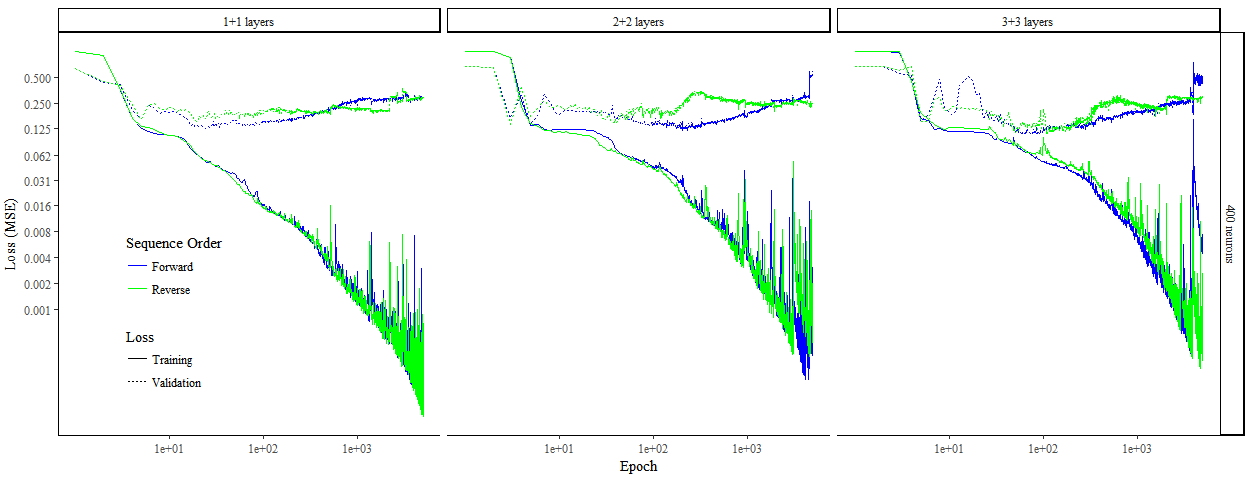
\includegraphics[width=1\textwidth]{reverse.PNG}
	\caption{Effects of sequence reversal on the training and validation losses. Three sets of models were trained, each has different number of hidden layer in the encoder-decoder structure. All models have \(400\) neurons in each hidden layer. Models were trained with Adam optimiser at \(B=256\) with no dropout.}
	\label{fig:reverse}
\end{figure}

Evidently, reversing input sequence has detrimental effect on the model’s validation loss. Despite the shapes of the training losses are very similar across all models, there is a considerable gap between the validation losses of forward and reverse models. Reverse models perform far worse in all scenarios as the validation MSEs are much larger.

When the sequence is reversed, the end of the input sequence is highly correlated with the output sequence’s beginning. This encourages the LSTM to overwrite previously learned information in the hidden recurrent state, which eventually sacrificing longer-term memory and worsened the model's loss. 

\subsubsection{Sequence Length}

For any given model with fixed number of layers and neurons, the sequence length \(T\) can be varied in order to show the effects of the seq2seq autoencoder. 

\begin{figure}[H]
	\centering
	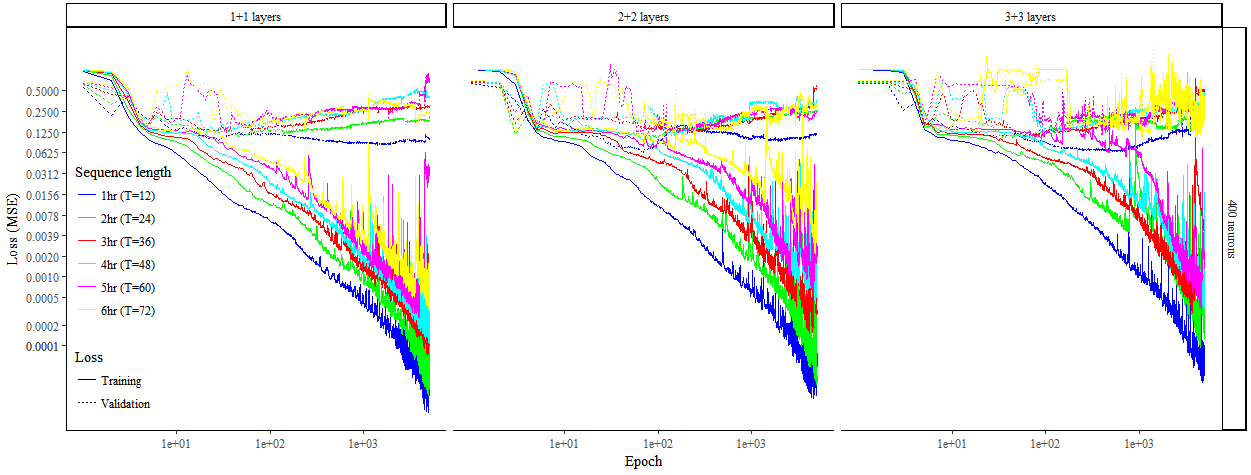
\includegraphics[width=1\textwidth]{sequence_length.PNG}
	\caption{Effect of sequence length on the training and validation MSE loss of three sets of models. All models were trained with Adam optimiser at \(B=256\) with no dropout.}
	\label{fig:sequence_length}
\end{figure}

In figure \ref{fig:sequence_length}, there is a clear pattern where models with shorter sequence length \(T\) have the smallest training and validation loss. The MSE goes up when the sequence length \(T\) is increased.

In theory, shorter sequences can be more effectively encoded into context representation as they contain less information. While on the other hand, longer sequences naturally contains more information. Cho et al. \cite{cho2014b} studied the effects of sequence length in machine translation and also concluded that the context vector becomes bottleneck when handling long sequences. This suggests that the RNN encode-decoder structure requires more memory capacity in order to handle long sequences successfully.

\subsubsection{Sequence Reconstruction}

The decoder structure reads the fixed-length context vector and translate it into the target sequence. Here we can select one model and closely examine the predictions qualitatively by visualisation.

A deep autoencoder model with \(3+3\) layers and \(400\) neurons was selected. It was trained using Adam optimiser for \(5000\) epochs with \(0.4\) dropout rate. The decoder output which contains \(K=6\) dimensions with sequence length \(T=36\) is visualised as heatmap in figure \ref{fig:heatmaps} below.

\begin{figure}[H]
	\centering
	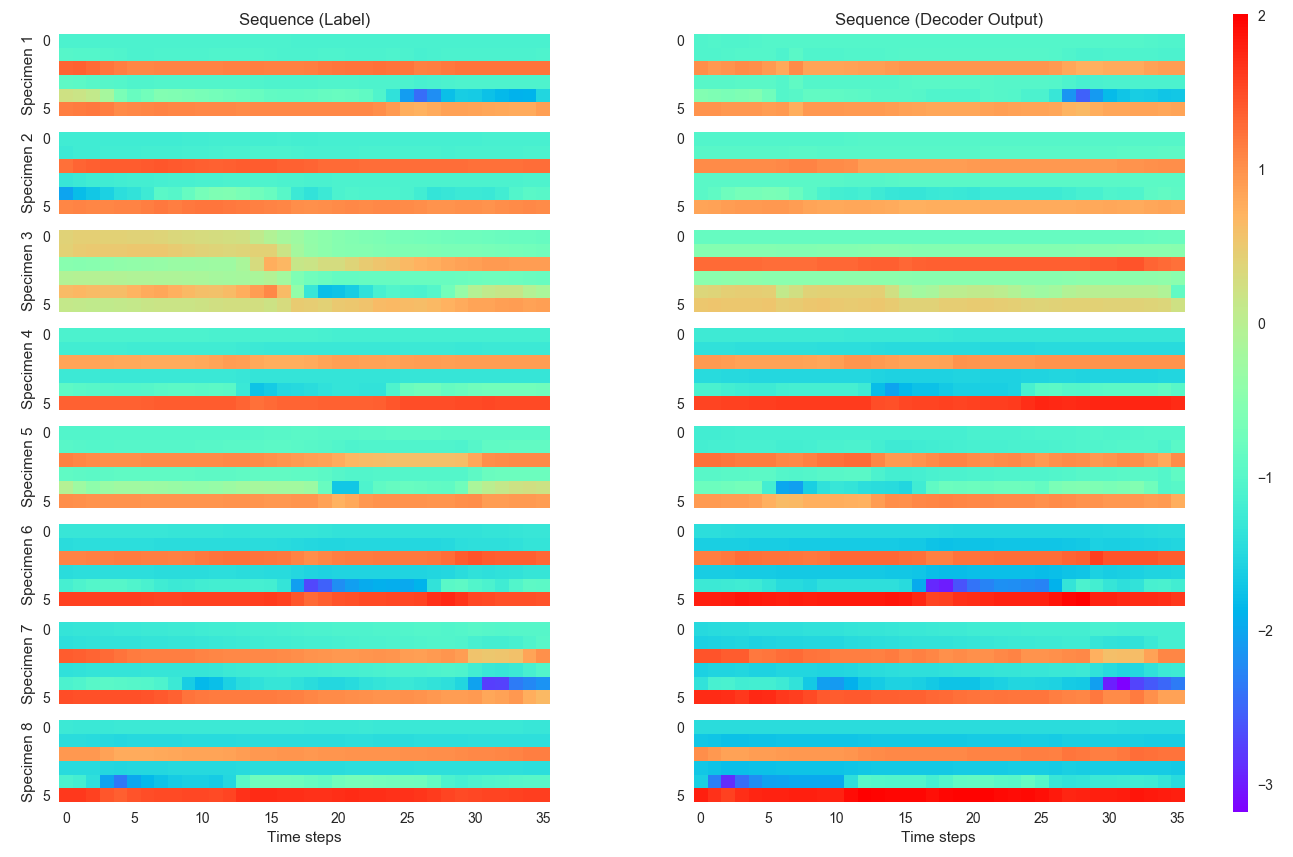
\includegraphics[width=1\textwidth]{heatmaps.PNG}
	\caption{A heatmap showing eight randomly selected output sequences in the held-out validation set. Colour represents magnitude of sensor measurements in normalised scale.}
	\label{fig:heatmaps}
\end{figure}

Through qualitative inspection, we can see that all the selected specimens demonstrate sufficient similarity between the original label and the decoder output. The model clearly captures both the mean level as well as temporal variations of all the dimensions. This suggests that the model is capable of generalising its knowledge to unseen validation data.

\subsection{Analysing Context Vector}

Once the seq2seq autoencoder model is successfully trained, the fixed-length context vectors were extracted from the model and examined in greater details. Following the example in previous section, the same model was used to extract context vectors. 

As we discussed earlier, successive context vectors have similar activation as they are only shifted by one time step. By calculating the correlation matrix of all context vectors and visualising them on a heatmap as in figure \ref{fig:matrix}, it is found that the band around the diagonal has higher correlation. This shows that nearby context vectors are highly correlated.

\begin{figure}[H]
	\centering
	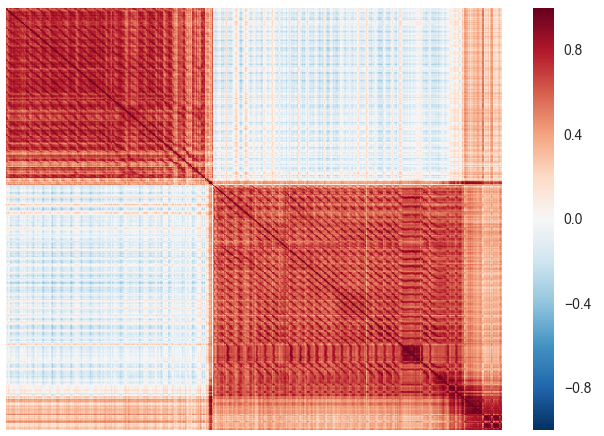
\includegraphics[width=0.7\textwidth]{matrix.PNG}
	\caption{A correlation matrix showing the pairwise correlation of all context vectors. Notice the narrow band around the diagonal always has strong correlation.}
	\label{fig:matrix}
\end{figure}

In the model we selected, the context vector \(c\) is a \(400\)-dimensional vector \(\mathbb{R}^{400}\). Dimensionality reduction of the context vectors through principal component analysis (PCA) reveals that context vectors can be efficiently embedded in lower dimensions (e.g. two-dimensional space). 

At the lower dimensional space, we can use supervised classification algorithms to learn the relationship between vectors representations and cluster assignment. The trained classification model can then be applied to the validation set to predict clusters of any unseen data. In our experiment, a SVM classifier with radial basis function (RBF) kernel (\(\gamma=4\)) was used. This is shown in figure \ref{fig:pca_cluster} below.

\begin{figure}[H]
	\centering
	
	\begin{subfigure}[b]{0.48\textwidth}
		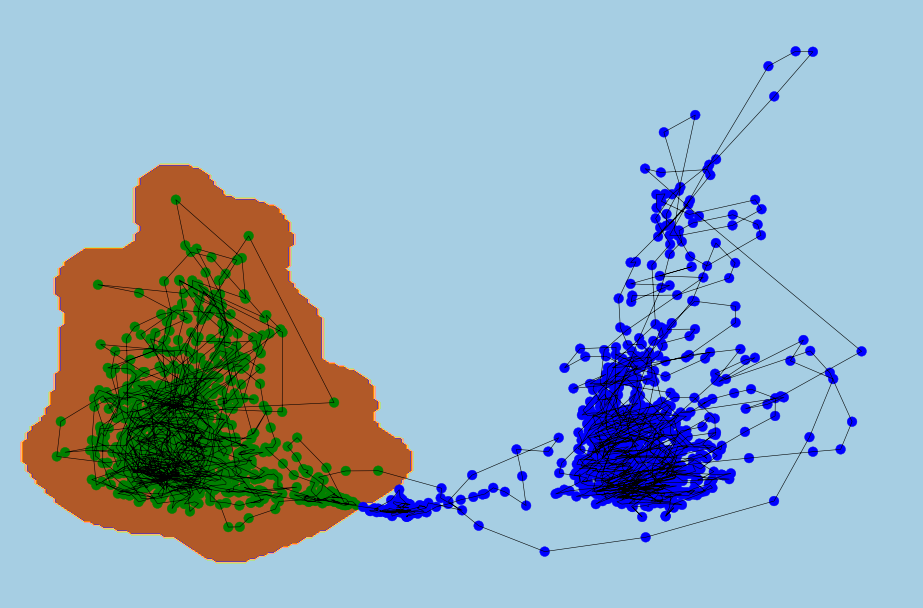
\includegraphics[width=\textwidth]{pca_cluster_2.PNG}
		\caption{\(2\) clusters}
		\label{fig:pca_cluster_2}
	\end{subfigure}
	~
	\begin{subfigure}[b]{0.48\textwidth}
		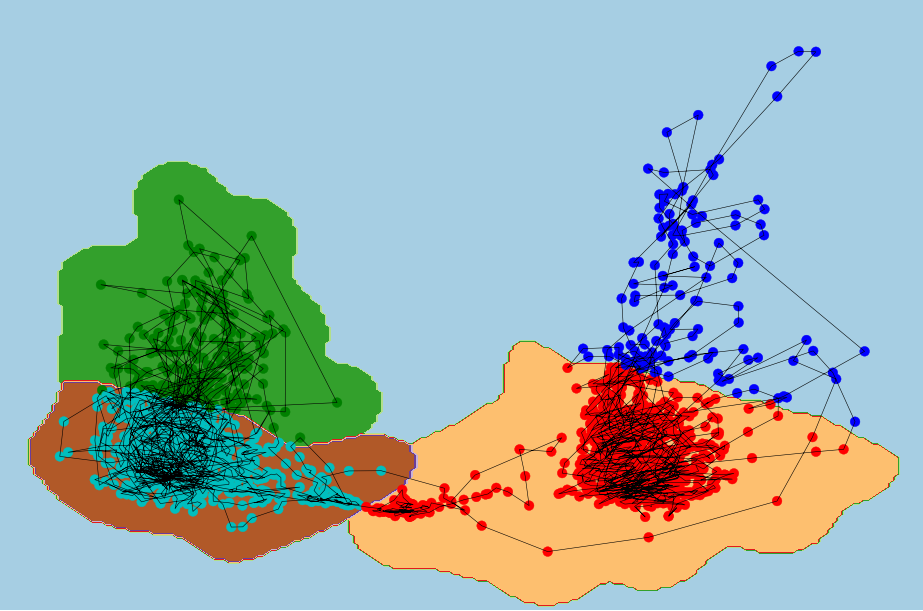
\includegraphics[width=\textwidth]{pca_cluster_4.PNG}
		\caption{\(4\) clusters}
		\label{fig:pca_cluster_4}
	\end{subfigure}

	\begin{subfigure}[b]{0.48\textwidth}
		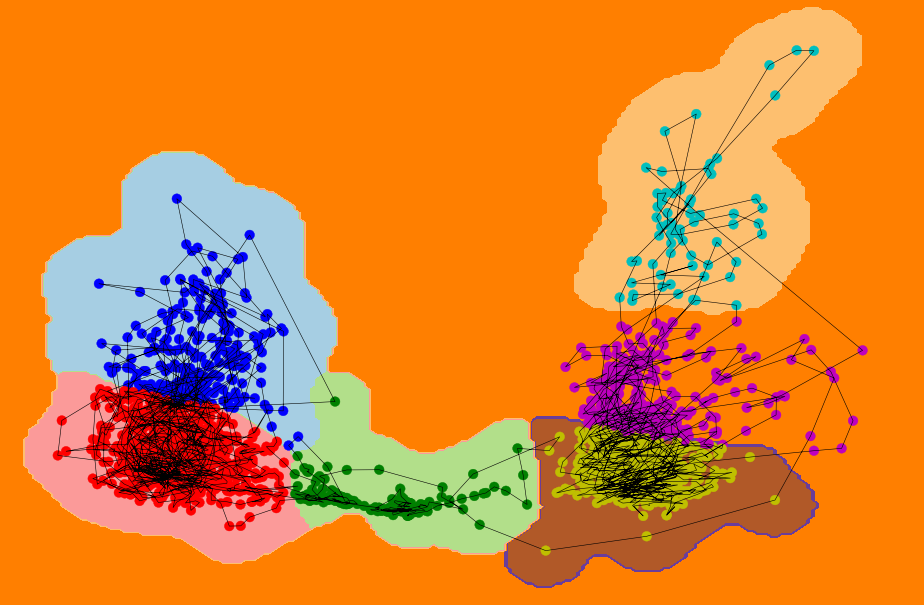
\includegraphics[width=\textwidth]{pca_cluster_6.PNG}
		\caption{\(6\) clusters}
		\label{fig:pca_cluster_6}
	\end{subfigure}
	~
	\begin{subfigure}[b]{0.48\textwidth}
		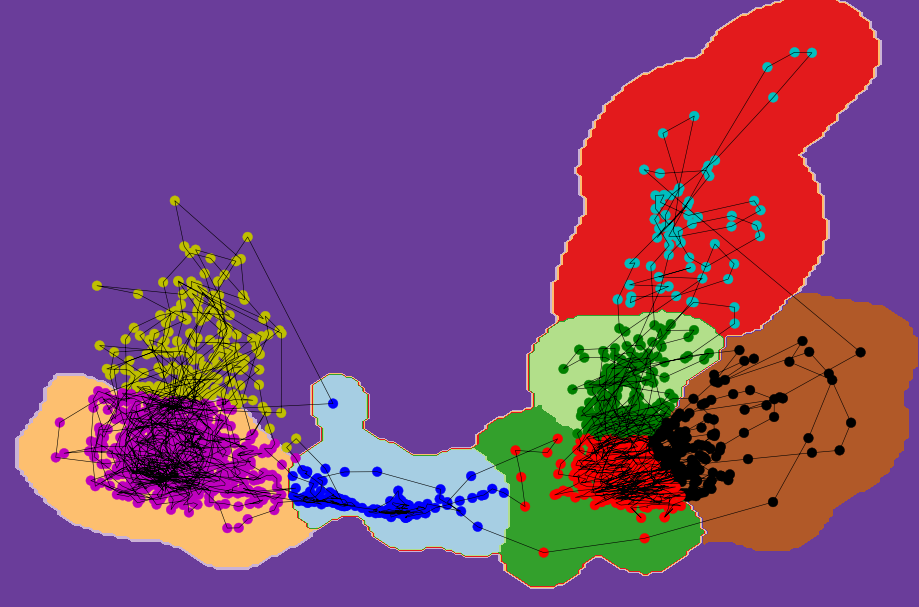
\includegraphics[width=\textwidth]{pca_cluster_7.PNG}
		\caption{\(7\) clusters}
		\label{fig:pca_cluster_7}
	\end{subfigure}

	\caption{Both training and validation sets were fed to the model and the context vectors were extracted. The context vectors were projected into two-dimensional space using PCA. The black solid line joins all consecutive context vectors together as a travelling path. Different number of clusters were identified using simple \(K\)-means algorithm. Clusters and the SVM decision boundaries are coloured in the charts.}
	
	\label{fig:pca_cluster}
\end{figure}

In order to understand the meaning of the context vectors, the output dimensions are visualised on a time axis in figure \ref{fig:context_timeline} below. The lines are colour-coded so that they can be matched to the corresponding clusters in figure \ref{fig:pca_cluster}.

\begin{figure}[H]
	\centering
	
	\begin{subfigure}[b]{0.4\textwidth}
		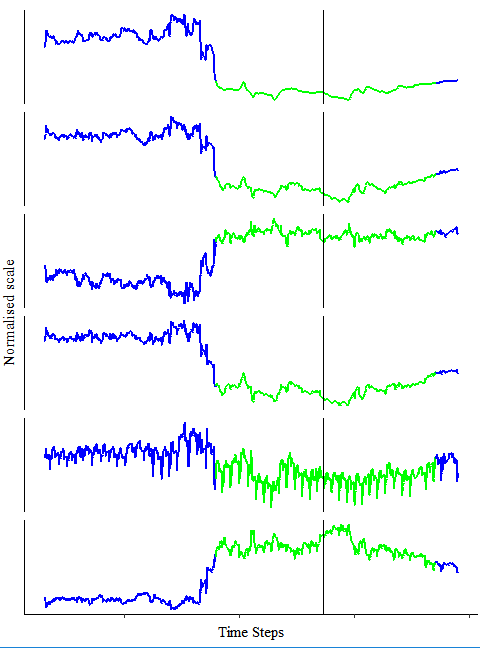
\includegraphics[width=\textwidth]{context_timeline_2.PNG}
		\caption{\(2\) clusters}
		\label{fig:context_timeline_2}
	\end{subfigure}
	~
	\begin{subfigure}[b]{0.4\textwidth}
		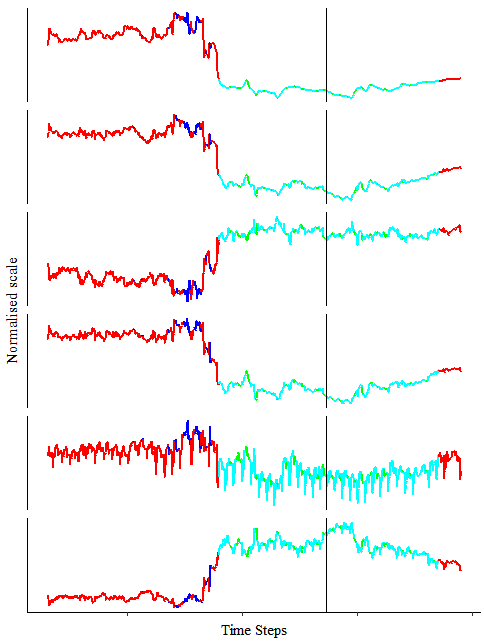
\includegraphics[width=\textwidth]{context_timeline_4.PNG}
		\caption{\(4\) clusters}
		\label{fig:context_timeline_4}
	\end{subfigure}
	
	\begin{subfigure}[b]{0.4\textwidth}
		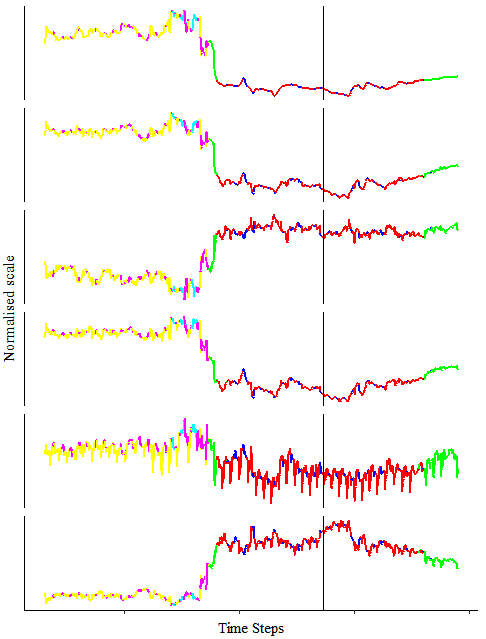
\includegraphics[width=\textwidth]{context_timeline_6.PNG}
		\caption{\(6\) clusters}
		\label{fig:context_timeline_6}
	\end{subfigure}
	~
	\begin{subfigure}[b]{0.4\textwidth}
		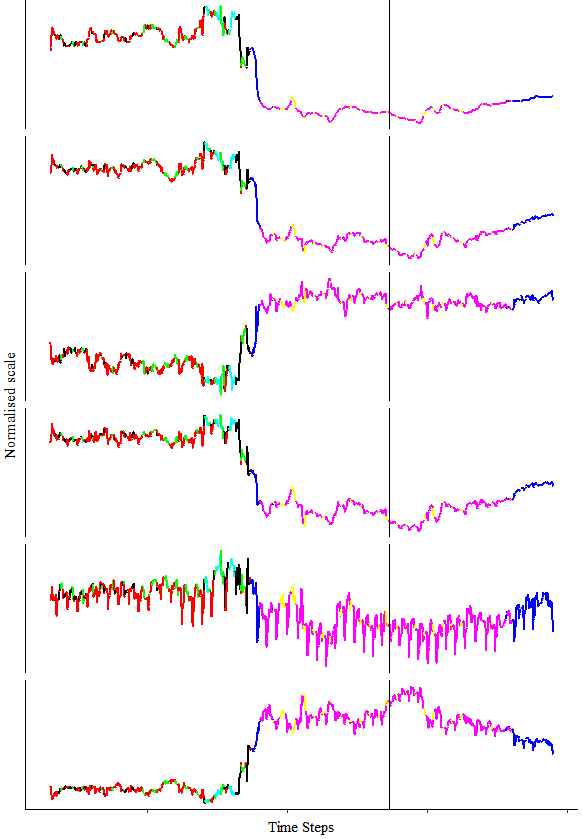
\includegraphics[width=\textwidth]{context_timeline_7.PNG}
		\caption{\(7\) clusters}
		\label{fig:context_timeline_7}
	\end{subfigure}

	\caption{Output dimensions are visualised on a shared time axis. The black solid line demarcates the training set (\(70\%\)) and validation sets (\(30\%\)). The line segments are colour-coded to match the clusters in the previous figure.}
	\label{fig:context_timeline}
\end{figure}

The context vectors are able to extract meaningful features from the sequence. In the two-dimensional space, the context vectors separate into two clearly identifiable neighbourhoods which correspond to the shift in mean values across all dimensions. When \(K\)-means clustering algorithm is applied, it captures these two neighbourhoods as two clusters in the first scenario.

When the number of clusters increases, they begin to capture more subtle variations. For instance, the context vectors coloured in deep blue in the \(4\) clusters scenario correspond to extreme values across different dimensions. At the same time, the cyan cluster reflects deep troughs in the fifth dimension. This indicates the recurrent autoencoder model is capable of encoding temporal patterns into a fixed-length vector representation.

When the number of clusters is further increased, even more details are captured. In the \(6\) clusters scenario, successive context vectors travel back and forth between the yellow and magenta cluster. This is also apparently driven by the oscillation of the fifth dimension. When the mean level begins to shift, the context travels between the red/blue clusters instead. Such pattern can also be observed in the validation set, which indicate that the knowledge learned by the autoencoder model is generalisable. When the number of cluster is increased to \(7\), consistent behaviour can still be observed.

Furthermore, the clusters can be closely examined by extracting the mean values of each dimension along the sequence and grouped by clusters. Figure \ref{fig:cluster_boxplot} illustrates all the dimensions of the \(6\) clusters scenario. Again, it shows that clusters are able to capture different temporal patterns. For instance, We already know that the context vectors drifts between the magenta/yellow clusters and red/blue clusters. The dimensional mean values of these cluster pairs have substantially different shapes. 

\begin{figure}[H]
	\centering
	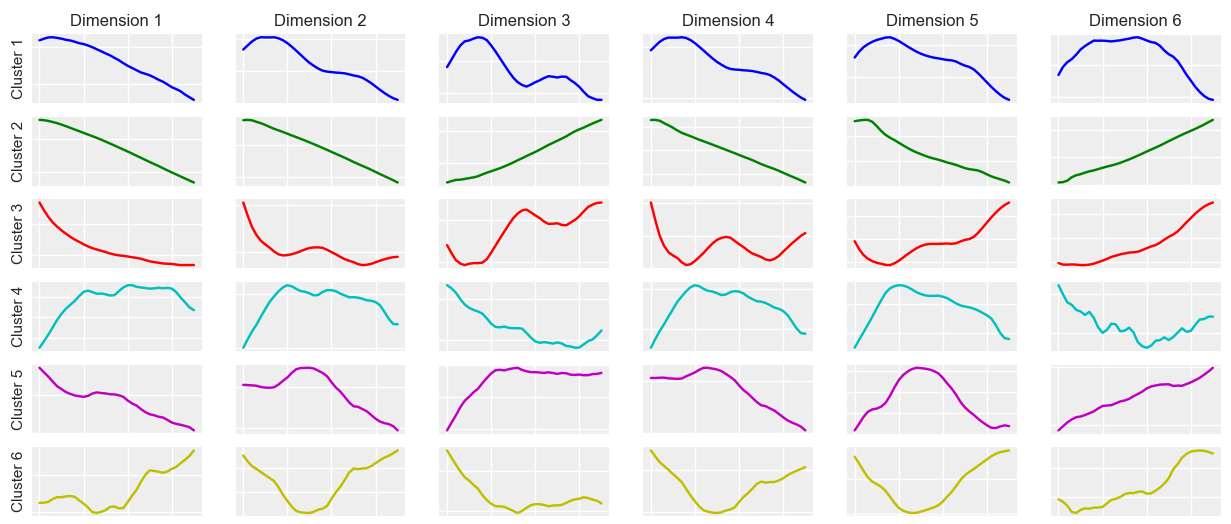
\includegraphics[width=0.95\textwidth]{cluster_boxplot.PNG}
	\caption{Showing the mean value of each dimension of the \(6\) clusters scenario. The horizontal axis is the time step where \(T=36\).}
	\label{fig:cluster_boxplot}
\end{figure}


\subsubsection {Alternative Example}

We have applied the seq2seq autoencoder model to a different set of selected sensors and analysed the results. This set contains only two sensors (\(P=158; K=2\)) which measures a specific aspect of the system process. The context vectors were extracted for further examination.

\begin{figure}[H]
	\centering
	
	\begin{subfigure}[b]{0.48\textwidth}
		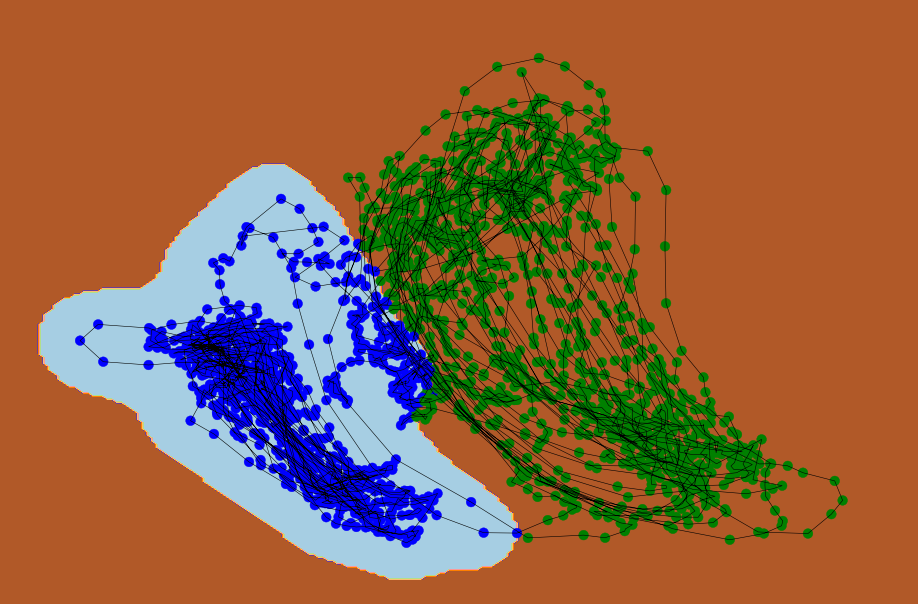
\includegraphics[width=\textwidth]{ex2_pca_cluster_2.PNG}
		\caption{\(2\) clusters}
		\label{fig:ex2_pca_cluster_2}
	\end{subfigure}
	~
	\begin{subfigure}[b]{0.48\textwidth}
		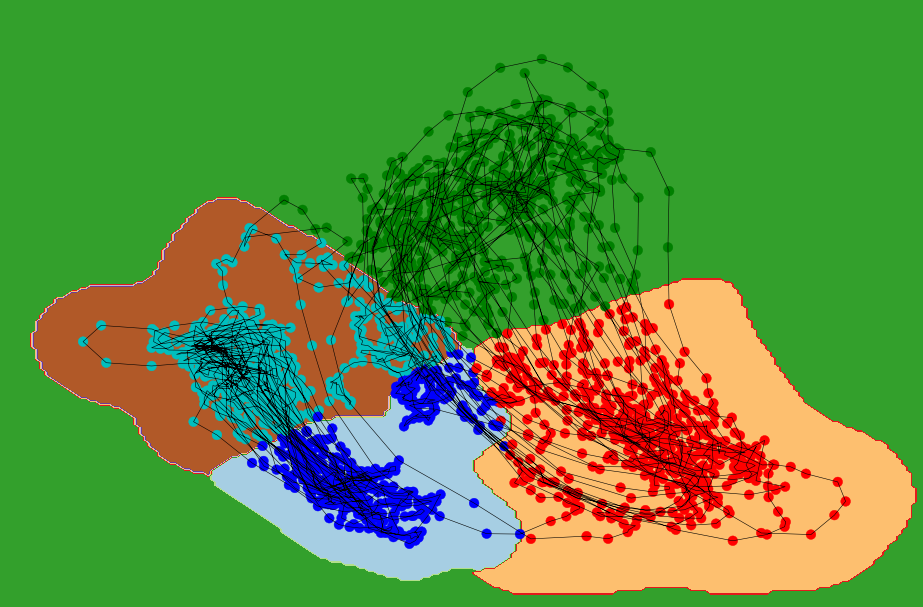
\includegraphics[width=\textwidth]{ex2_pca_cluster_4.PNG}
		\caption{\(4\) clusters}
		\label{fig:ex2_pca_cluster_4}
	\end{subfigure}
	
	\begin{subfigure}[b]{0.48\textwidth}
		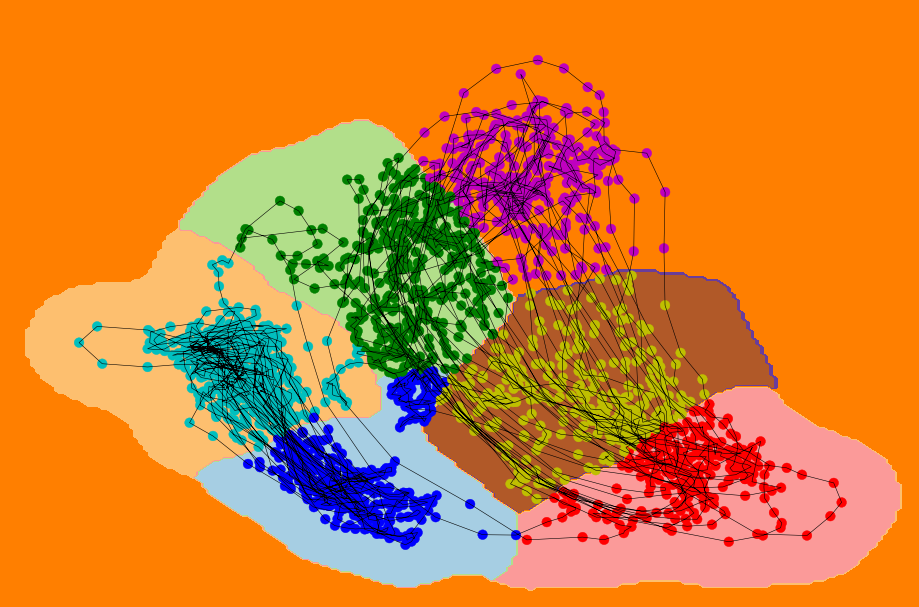
\includegraphics[width=\textwidth]{ex2_pca_cluster_6.PNG}
		\caption{\(6\) clusters}
		\label{fig:ex2_pca_cluster_6}
	\end{subfigure}
	~
	\begin{subfigure}[b]{0.48\textwidth}
		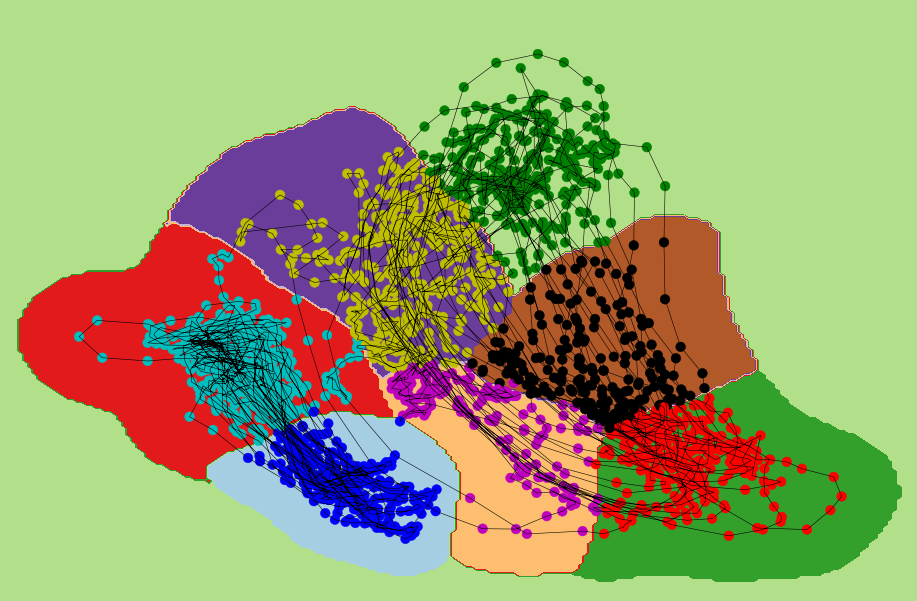
\includegraphics[width=\textwidth]{ex2_pca_cluster_7.PNG}
		\caption{\(7\) clusters}
		\label{fig:ex2_pca_cluster_7}
	\end{subfigure}
	
	\caption{Context vectors visualised in two-dimensional space via PCA. Various numbers of clusters were identified using \(K\)-means algorithm. The decision boundary was trained by SVM with RBF kernel.}
	
	\label{fig:ex2_pca_cluster}
\end{figure}

Successive context vectors form a smooth travelling path in the charts above. The context vectors drifts within a neighbourhood when the sequences have similar activation. They travel away from the original neighbourhood when activations becomes sufficiently different. Measurement of both output dimensions are visualised in figure\ref{fig:ex2_context_timeline} below, the colour can be mapped to the cluster of the context vectors in figure \ref{fig:ex2_pca_cluster}.

\begin{figure}[H]
	\centering
	
	\begin{subfigure}[b]{0.4\textwidth}
		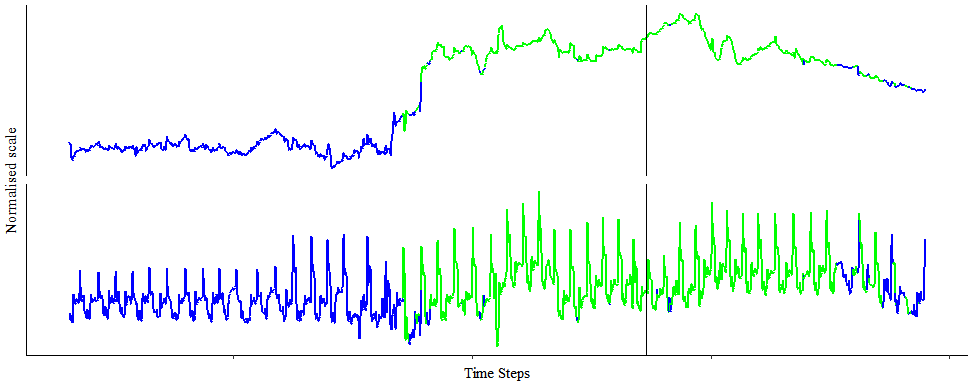
\includegraphics[width=\textwidth]{ex2_context_timeline_2.PNG}
		\caption{\(2\) clusters}
		\label{fig:ex2_context_timeline_2}
	\end{subfigure}
	~
	\begin{subfigure}[b]{0.4\textwidth}
		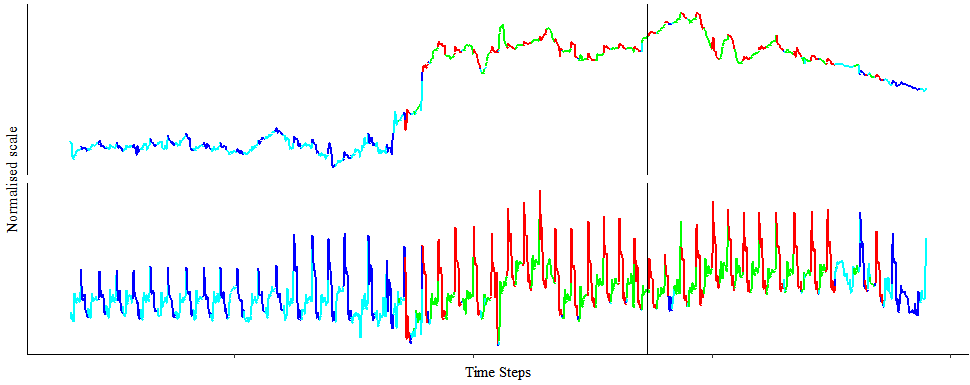
\includegraphics[width=\textwidth]{ex2_context_timeline_4.PNG}
		\caption{\(4\) clusters}
		\label{fig:ex2_context_timeline_4}
	\end{subfigure}
	
	\begin{subfigure}[b]{0.4\textwidth}
		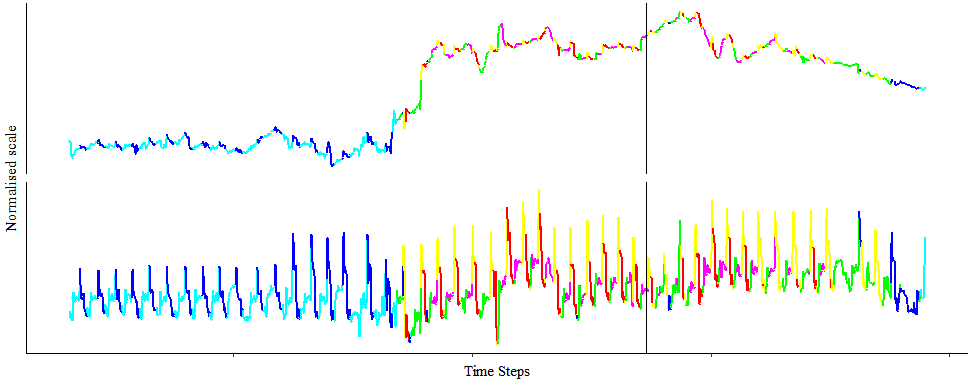
\includegraphics[width=\textwidth]{ex2_context_timeline_6.PNG}
		\caption{\(6\) clusters}
		\label{fig:ex2_context_timeline_6}
	\end{subfigure}
	~
	\begin{subfigure}[b]{0.4\textwidth}
		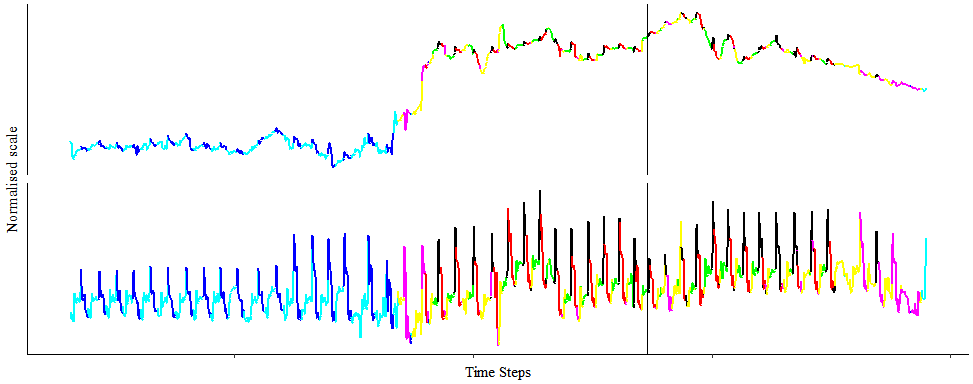
\includegraphics[width=\textwidth]{ex2_context_timeline_7.PNG}
		\caption{\(7\) clusters}
		\label{fig:ex2_context_timeline_7}
	\end{subfigure}
	
	\caption{Output dimensions visualised on a time axis. The training set (\(70\%\)) and validation set (\(30\%\)) are demarcated by the black solid line. Line colour can be matched to the corresponding cluster in figure \ref{fig:ex2_pca_cluster}}.
	\label{fig:ex2_context_timeline}
\end{figure}

As we can see in this example, the context vector is also able to capture temporal patterns efficiently. For instance, the context vectors in the \(2\) clusters can separate level shift of the sequence. While in the \(4\) clusters scenario, the context vectors located in the red/blue clusters correspond well to a falling edge  in the second dimension and the remaining clusters correspond to a rising edge.

\newpage
\section{Discussion}

In this study, we have described how seq2seq model can be adapted into recurrent autoencoder setting. Multiple streams of sensor values can be fed to the autoencoder model by treating them as a multidimensional sequence. The encoder structure compresses the entire input sequence into a fixed-length context vector which is conditional on the decoder's output. We have extracted context vectors and analysed its properties in details. 

One of the key contribution of this study is that sequences can be generated recursively by shifting one time step. Successive context vectors generated in this way are always highly correlated, thus form a travelling path in high dimensional space. Dimensionality reduction techniques and clustering algorithms were applied to aid visualisation. Such property can be used to create diagnostic measurements for large-scale industrial process. 
 
When the sensor values are fed to seq2seq model as multidimensional sequence, it gets compressed into a context vector which drifts within a neighbourhood. A decision boundary can be imposed (e.g. one-class SVM) to define the neighbourhood boundary of the normal healthy state. The seq2seq autoencoder model can be applied in an on-line setting which allows diagnostic measurements to be generated with real-time data. For instance, alert can be triggered when the context vector travels beyond the known healthy neighbourhood. This idea is illustrated in figure \ref{fig:contexttravel} below. 

For more dynamic processes, sensor measurement may fluctuate at multiple ranges with transition between multiple states. This study used a large-scale two-stage compression train to illustrate this case. The movement of context vectors can be used to create meaningful diagnostic measurement, such as when the system changes from one state to another. This is illustrated in figure \ref{fig:contexttravel2}.

\begin{figure}[H]
	\centering
	\begin{subfigure}[b]{0.35\textwidth}
		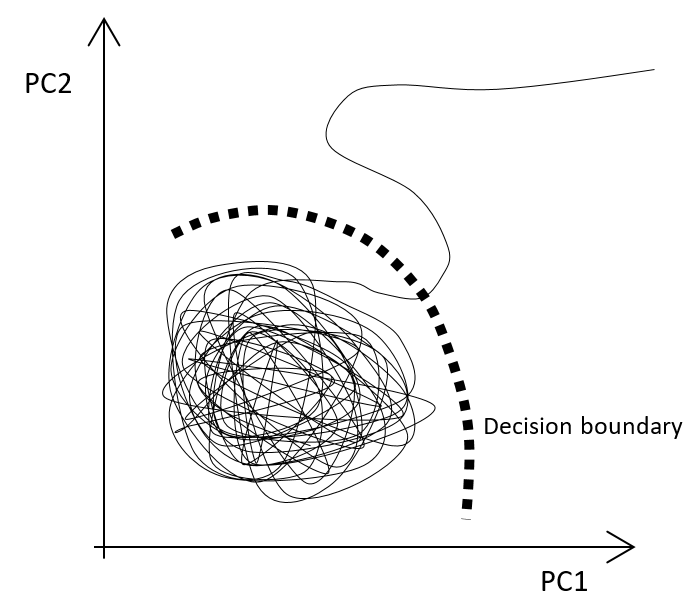
\includegraphics[width=\textwidth]{contexttravel.PNG}
		\caption{Process with a single healthy state.}
		\label{fig:contexttravel}
	\end{subfigure}
	~
	\begin{subfigure}[b]{0.35\textwidth}
		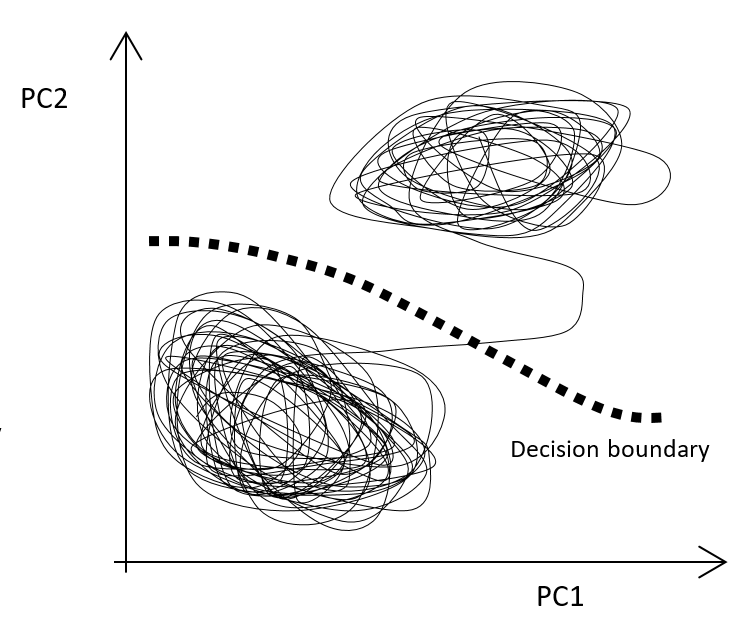
\includegraphics[width=\textwidth]{contexttravel2.PNG}
		\caption{Multi-state process with transition between states.}
		\label{fig:contexttravel2}
	\end{subfigure}
	\caption{Travelling context vector.}
\end{figure}

This study also proposed dimensionality relaxation which allows the autoencoder model to produce partial reconstruction of the input sequence. It makes more information available and allows the context layer to summarise the input sequence conditionally based on the corresponding output.

The seq2seq autoencoder model can be applied to any multi-sensor multi-state processes. For example, it can be extended to vehicle telematics or Human Activity Recognition in an on-line setting using pre-trained models. Alerts can be triggered when the context vector drifts away from a known neighbourhood, or when it travel between two known neighbourhoods (i.e. state transition).

\subsection{Professional Issues}

History of the gas terminal goes back to the 1990s and the production facility went through upgrades and modifications from time to time. Due to this reason, sensor data recorded through time does not necessarily reflect the same underlying process state.

The dataset was collected across several years but the quality of archived data is very inconsistent. Sensor measurements have been recorded at precise time at millisecond level but the subsecond portion of the date/time tag was removed due to data type constraints in the archive system. This resulted in the permanent loss of the original date/time tag and contributed to unequally-spaced observations.

Moreover, there are tens of thousands of sensors installed at the production site, both onshore and offshore, as well as at subsurface level. The sensor data was archived on several legacy databases. This study only covers a small subset of sensors located at the two-stage gas compression train which were extracted from a single archive system. This implies that sensors at other locations are out-of-scope. It is possible that expanding the set of sensors may help improve model loss (e.g. by including more lead variables). Nevertheless, categorical sensor data (e.g. open/closed, tripped/healthy, start/stop... etc) were not included in this study. These may help provide directions for future research.

This proprietary dataset is provided by Centrica PLC (Registered office address: Millstream Maidenhead Road, Windsor, Berkshire, SL4 5GD) with all rights reserved. This study was supported by the same company especially with assistance from the Exploration and Production division based in Aberdeen, Scotland.

\subsubsection{Self-Assessment}

In earlier phases of the project, various ideas were experimented before committing to the current path. The initial idea was to apply RNN at \(t\) and make predictions for one step ahead at \(t+1\). When this was applied recursively through time, the loss amplifies massively therefore rendering the predictions useless. Since then a lot of time was spent on background research.

Another ideas we previously experimented was to use seq2seq model to make predictions at multiple steps ahead. This means feeding multidimensional sequence at \(t=\{1,2,3,...,T\}\) to the encoder and make the decoder to output the sequence at \(t=\{T+1,T+2,T+3,...T+h\}\) where \(h\) is the number of steps ahead we want to forecast.

This ideas actually works fairly well on sensors with strong seasonality. The RNN encoder-decoder structure was able to capture repeating patterns at multiple steps ahead. However it fails to make prediction when the signal varies but without clear pattern. This could be due to the lack of lead sensor measurements which makes multi-steps ahead forecast particularly challenging. However the idea was never substantiated as we did not further pursue along this research direction.

The eventual deliverable of this study was to modify the previous idea into an autoencoder setting, simply by aligning the time steps of the input and output sequences. This path was found to be more promising. A lot of analysis including strong emphasis on visualisation and clustering were included in this report.

A major challenge throughout the entire project was the training of ANN models. Gradient-based training is very slow despite already having access to good quality hardware. Determining the optimal hyperparameters is extremely hard since exhaustive search is almost impossible. The effects of certain hyperparameters were tested with arbitrarily selected values, such as the number of layers where only \(1+1\), \(2+2\) and \(3+3\) layers structures were tested. The effects of even deeper models were not experimented within the scope of this study. Furthermore, the hyperparameters of ANNs are data-specific which means that it must be adapted when the dataset is changed.

Nevertheless, improvements can be made to the seq2seq model but were not further investigated within the scope of this study. When we experiment the effect of sequence reversal, only forward and reversed sequences were tested. It is actually possible to combine both orders at the same time by using bidirectional RNN (BRNN). It is suspected that the BRNN-based encoder would outperform either forward or reverse RNN. It was not experimented because it requires substantial code modification which the project's schedule cannot accommodate.

\newpage
\begin{appendices}
	
	\section{Activation Functions}
	
	In an ANN, each hidden neuron carries a non-linear activation function \(f(x)\). Sigmoid function is a traditional choice of activation function for ANNs. It takes the weighted sum of input plus the bias unit and squashes everything into the range \((0,1)\) with a characteristic sigmoidal ‘S’ shape. Cybenko \cite{cybenko} has suggested that sigmoid function can be powerfully used as universal approximator for any continuous non-linear function. This is later known as the universal approximation theorem. As the sigmoid function is differentiable and easy to compute, it soon becomes a popular choice for ANN activation function. However, it suffers from weak gradient when the input is far away from zero (i.e. the neuron saturates), which makes the ANN learn very slow. 
	
	Given that ANNs are trained via backpropagation which is a gradient descent technique, activation functions which provide stronger gradient are usually preferred. This means the choice of the ANN’s activation function bears profound implication on the gradient and hence the network’s general ability to train and learn. 
	
	To address the problem of weak gradient, alternative activation functions have been proposed. For instance, the hyperbolic tangent can be used. It shares the same sigmoidal shape but further stretches the output to the range \((-1,1)\) therefore provides stronger gradient. Yet, the gradient still suffers from saturation when the input is too small or too large.
	
	Different activation functions can provide stronger gradients while maintaining non-linearity. For instance, the softplus function has strong gradient (i.e. unsaturable) for any positive input \cite{françois}. However, it has been considered computationally costly as it contains logarithm and exponential terms. In light of this, a simplified version call rectified linear unit (ReLU) is usually used instead \cite{hahnloser}. The shape of ReLU is very similar to softplus with the exception that it has a threshold at zero. This means only positive input can lead to activation. However, the weighted sum input can change to negative value during training therefore causing the ReLU neuron to cease training. This is called the dying ReLU problem. To avoid this, a very small gradient can be introduced to the negative range to allow the neuron to recover. Such idea is embodied in implementations such as leaky ReLU \cite{maas} and Parameterised ReLU (PReLU) \cite{he}.
	
	\begin{subequations}
		Sigmoid activation
		\begin{equation}
		\label{sigmoid}
		f(x)= \frac{1}{1+e^{-x}}
		\end{equation}
		
		Hyperbolic tangent activation
		\begin{equation}
		\label{tanh}
		f(x)= \frac{e^x-e^{-x}}{e^x+e^{-x}}
		\end{equation}
		
		Softplus activation
		\begin{equation}
		\label{softplus}
		f(x)= \ln(1+e^x)
		\end{equation}
		
		Rectified linear unit (ReLU)
		\begin{equation}
		\label{relu}
		f(x)= \max(0,x)
		\end{equation}
		
		Leaky ReLU
		\begin{equation}
		\label{leaky}
		f(x)= \begin{cases}
		0.001x\\
		x
		\end{cases}
		\end{equation}
		
		Parametrised ReLU (PReLU)
		\begin{equation}
		\label{prelu}
		f(x)= \begin{cases}
		ax\\
		x
		\end{cases}
		\end{equation}
		
	\end{subequations}
	
	The output prediction is made at the network's final layer. Each neuron at this layer combines the hidden neuron's activation though weighted sum and a bias adjustment unit \eqref{weightedhidden}. For regression problems, a linear activation layer is usually used to map the output vector back into unbounded real value range \eqref{linear}. For classification problem, softmax function is used as the final output layer. It maps the hidden layer’s activations into the range \((0,1)\) where the sum of the entire output vector is restricted to\(1\) in order to represent class probabilities \eqref{softmax}.
	
	\begin{subequations}
		Weighted sum of hidden vector with bias adjustment
		\begin{equation}
		\label{weightedhidden}
		y_k=b_k+\sum_{h=1}^{H} w_{h,k}h_h , k=1,...,K
		\end{equation}
		
		Linear output
		\begin{equation}
		\label{linear}
		\hat{Y_k} = y_k
		\end{equation}
				
		Softmax output
		\begin{equation}
		\label{softmax}
		\hat{Y_k} = \frac{e^{y_k}}{ \sum_{k^\prime=1}^{K} e^{y_{k^\prime}} }
		\end{equation}
	\end{subequations}

\newpage
	\section{Optimisation}
	ANNs are capable of learning complex behaviours through non-linear activation functions with a set of learnable parameters. It essentially performs vector mapping  \(f: \mathbb{R}^P\rightarrow\mathbb{R}^K \)) with a loss function \(\mathcal{L}\) representing the quality of the prediction. The goal of optimisation is to find a set of model parameters which minimises the ANN’s loss function.
	
	\subsection{Batch Gradient Descent}
	In a modern ANN, gradient-based technique lays the foundation of optimisation methods. We can illustrate the concept using a simple ANN which takes a set of model parameters denoted as w and loss function \(\mathcal{L}_w\). The gradient of the loss function \(\nabla\mathcal{L}_w\) is the differentiation of the loss \(\mathcal{L}_w\) with respect to the parameter \(w\). It basically indicates the instantaneous change of loss when \(w\) shifts by an incredibly small amount. To improve the loss function, the gradient is multiplied with a small learning rate \(\mu\) and subtracted from the original parameter \(w\). In this way, the parameter improves by descending through the direction of improvement as indicated by the gradient.
	
	\begin{subequations} 
		
		Evaluate gradient
		\begin{equation}
		\label{bgd1}
		\nabla\mathcal{L}_w=\lim\limits_{h\rightarrow 0}\frac{f(w+h)-f(w)}{h}
		\end{equation}
		
		Update gradient
		\begin{equation}
		\label{bgd2}
		w^\prime=w-\mu\nabla\mathcal{L}_w
		\end{equation}
		
	\end{subequations}
	
	\begin{algorithm}[H]
		\caption{Batch gradient descent}
		\label{bgd}
		
		\SetKwInOut{Input}{Input}
		\Input{Sample size \(N\)}
		
		\While{true}{
			Evaluate gradient with entire sample \(N\)\;
			Update gradient\;
		}
	\end{algorithm}
	
	For basic implementation of gradient descent optimiser, it is common to take the whole batch of sample and evaluate the gradient in every epoch. It is therefore slow and becomes inefficient for large datasets. Besides, the learning rate μ which decides the magnitude of each descent is predetermined. If \(\mu\) is too small, the parameter only descents by an exceedingly small step in every update. This usually results in very slow training in the beginning as the steps are small. Yet, smaller steps may help the parameter to reach optimal position in later part of the learning process. Contrarily, high learning rate implies bigger steps during gradient descent. This suggests faster learning in early training process, but the parameters may diverge from optima due to overshooting. Picking the correct learning rate has become a dilemma and has motivated many improvements of the original gradient descent algorithm.
	
	\subsection{Stochastic Gradient Descent}
	
	To address the problem of slow learning in batch gradient descent, a simple improvement is to evaluate the gradient with a single randomly selected sample. This is called stochastic gradient descent (SGD). 
	
	\begin{algorithm}[H]
		\label{sgd}
		\caption{Stochastic gradient descent}
		
		\SetKwInOut{Input}{Input}
		\Input{Sample size \(N\)}
		
		\While{true}{
			Shuffle sample \(N\)\;
			\ForEach{element \(n\in N\)}{
				Evaluate gradient with element \(n\)\;
				Update gradient\;
			}
		}
	\end{algorithm}
	
	As SGD performs gradient descent with just one sample drawn from the entire training set, the variance of the gradient can be unavoidably high. As the downhill gradient for one sample can be an uphill gradient for another sample, the gradient descent process can lead to heavy fluctuation of the parameter. Such behaviour has two-sided effects: On the positive side, fluctuations can avoid parameters being stuck at local optima. However, on the downside it may lead to It may lead to poor convergence at optimality as fluctuation endures.
	
	
	\subsection{Minibatch Gradient Descent}
	
	Minibatch is simply a special case of the SGD algorithm. It uses a batch of sample to evaluate loss gradient instead of just using a single sample. Variance of the gradient update is therefore lower than SGD which ultimately helps convergence while still permitting parameters to jump away from inferior positions.
	
	\begin{algorithm}[H]
		\label{minibatch}
		\caption{Minibatch gradient descent}
		
		\SetKwInOut{Input}{Input}
		\Input{Sample size \(N\)}
		\Input{Minibatch size \(B\)}
		
		\While{true}{
			Shuffle sample \(N\)\;
			
			\(i\leftarrow 0\)
			
			\While{\(i \leqslant \frac{N}{B}\) }{
				Draw a subset \((iB,  \min(N, (i+1)B)]\) from the sample\;
				Evaluate gradient with subset elements\;
				Update gradient\;
				\(i\leftarrow i+1\)
			}
		}
	\end{algorithm}
	
	
	\subsection{Momentum}
	
	Even though minibatch uses a batch sample to evaluate gradient, it still results in fluctuating gradients. Dampening the gradients can lead to faster training and better convergence. To achieve this, a momentum term is added to the gradient update. It takes a fixed portion α of the previous weight update and adds it to the current step. This helps the optimiser to navigate through a rough space by continuously descending towards minimum loss. In practice, the \(\alpha\) value is usually set at a high value such as \(\alpha=0.9\) in order to smooth out the descent movement.
	
	
	\begin{subequations} 
		
		Evaluate gradient
		\begin{equation}
		\label{momentum1}
		v_t=\alpha v_{t-1}+\mu \nabla \mathcal{L}_w
		\end{equation}
		
		Update gradient
		\begin{equation}
		\label{momentum2}
		w^\prime=w-v_t
		\end{equation}
		
	\end{subequations}
	
	\begin{figure}[H]
		\centering
		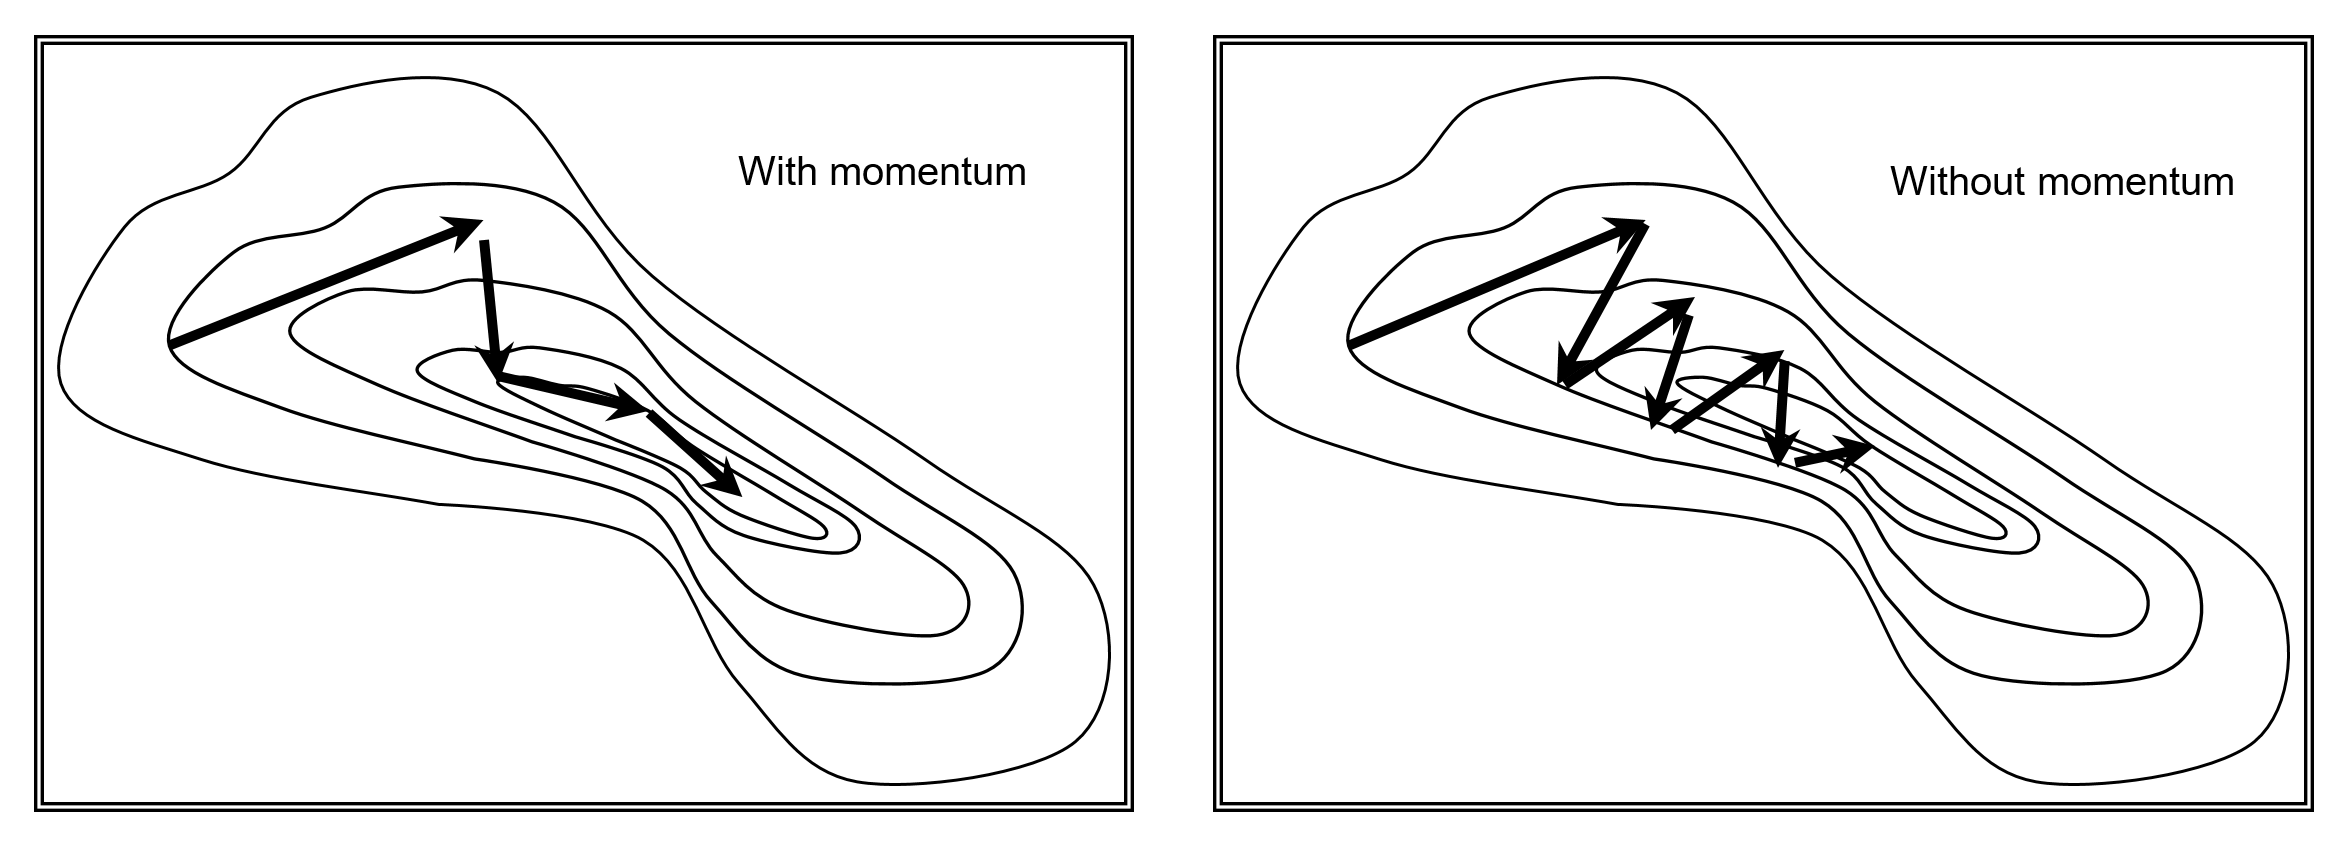
\includegraphics[width=1\textwidth]{momentum.PNG}
		\caption{Gradient descent with and without momentum}
		\label{fig:momentum}
	\end{figure}
	
	\subsection{Nesterov Momentum}
	
	Standard momentum shifts the parameter by inheriting a fixed portion from previous weight update. As this information is known prior to gradient evaluation, it can be incorporated with the existing parameter to give an approximation of the new position \cite{nesterov1983}. This is achieved by assessing the gradient at position \(w-\alpha v_{t-1}\) instead \eqref{nesterov1}. This approximated position is much closer to the locality of the new parameter as the momentum term is included, it therefore enables the gradient to look ahead at one further step. It then follows the standard momentum update rule \eqref{nesterov2} \eqref{nesterov3}.
	
	\begin{subequations} 
		
		Nesterov momentum
		\begin{equation}
		\label{nesterov1}
		w^{\prime\prime}=w-\alpha v_{t-1}
		\end{equation}
		
		
		Evaluate gradient
		\begin{equation}
		\label{nesterov2}
		v_t=\alpha v_{t-1}+\mu \nabla \mathcal{L}_{w^{\prime\prime}}
		\end{equation}
		
		Update gradient
		\begin{equation}
		\label{nesterov3}
		w^\prime=w-v_t
		\end{equation}
		
	\end{subequations}
	
	
	
	\subsection{Decay}
	
	For all the gradient descent algorithms described above, the learning rate \(\mu\) is a fixed global parameter which does not change throughout the optimisation process. It is easy to overshoot if the learning rate is too high. To avoid this, a rate of decay \(\omega\) can be applied to the learning rate so that the step size would decrease gradually and hence achieving better convergence. The \(\omega\) parameter is normally fixed at a small value such as \(\omega=10^{-6}\).
	
	Learning rate decay
	\begin{equation}
	\label{decay}
	\mu_t = \frac{\mu_{t-1}}{1+t\omega}
	\end{equation}
	
	
	\subsection{Adagrad}
	
	In a practical ANN, the number of trainable parameters can be very large. Adagrad optimiser provides adaptive learning rate for each parameter at every time step, which allows it to perform large update for parameters with higher gradients and vice versa \cite{duchi2011}.
	
	It modifies the learning rate μ by dividing it against the sum of square of the gradients of the past updates with respect to the parameter \eqref{adagrad1}. A small but positive term \(\epsilon\) is added to prevent division by zero \eqref{adagrad2}. For a parameter which experienced slow learning in the past (i.e. low gradient), the sum of square term \(g_t\) would be relatively small. This automatically scales the learning rate \(\mu\) to a larger value which speeds up optimisation in relation to this parameter. Contrastingly, the learning rate diminishes if the sum of square of the past gradients is large. 
	
	\begin{subequations} 	
		Sum of square term
		\begin{equation}
		\label{adagrad1}
		g_t=\sum_{t^\prime=1}^{t}(\nabla\mathcal{L}_{w,t^\prime})^2
		\end{equation}
		
		Update gradient
		\begin{equation}
		\label{adagrad2}
		w^\prime=w-\frac{\mu}{\sqrt{g_t}+\epsilon}\nabla\mathcal{L}_{w,t}
		\end{equation}
	\end{subequations}
	
	Adagrad accumulates past gradients in the denominator and it gets unavoidably large as training progresses. Ultimately the learning rate would become exceedingly small and leads to slow learning.
		
	\subsection{RMSprop}
	To address the shortcomings of Adagrad optimiser, the computation of the sum of square term \(g_t\) can be slightly modified. In an unpublished course material \cite{hinton2012unpub}, Hinton et al. suggests that the term should be made up of an exponentially decaying portion taken from the previous step and the rest being taken from the gradient at current step. The ratio \(\rho\) indicates the portion of exponentially decayed past squared gradients take from \(t-1\) \eqref{rmsprop1}. The authors suggest fixing the ratio at \(\rho=0.9\). The weight update formula of RMSprop is essentially the same as Adagrad except the \(g_t\) term is replaced by an exponentially decaying term. This effectively turns the sum of squared gradient into a moving average term which makes the learning rate more resilient from diminishing towards zero while maintaining responsiveness to recent gradients. 
	
	\begin{subequations} 
		
		Sum of square term
		\begin{equation}
		\label{rmsprop1}
		E[g_t]=\rho E[g_{t-1}]+(1-\rho)(\nabla \mathcal{L}_{w,t})^2
		\end{equation}
		
		Update gradient
		\begin{equation}
		\label{rmsprop2}
		w^\prime=w-\frac{\mu}{\sqrt{g_t}+\epsilon}\nabla \mathcal{L}_{w,t}
		\end{equation}
		
	\end{subequations}
	
	\subsection{Adam}
	
	Kingma \& Ba  \cite{kingma2014} proposed the Adam optimiser, which combines the concept of adaptive learning rate and momentum. It has parameters \(m_t\) and \(v_t\) which stores the decaying past gradient \eqref{adam1} and the decaying past squared gradient \eqref{adam2} respectively. These two terms are responsible of estimating the gradient’s mean and variance. As these parameters are initialised as zeros at the initial step, they are strongly inclined towards zero in most of the early weight update stages. In light of this, the bias adjusted values \(\hat{m}_t\) and \(\hat{v}_t\) are computed by dividing the unadjusted value over a logarithmically saturating term \eqref{adam3} \eqref{adam4}. The bias adjusted values are then used to compute the gradient update \eqref{adam5}.
	
	
	\begin{subequations} 
		
		Decaying past gradient
		\begin{equation}
		\label{adam1}
		m_t=\beta_1m_{t-1} + (1-\beta_1)\nabla \mathcal{L}_{w(t,i)}
		\end{equation}
		
		Decaying past squared gradient
		\begin{equation}
		\label{adam2}
		v_t=\beta_2 v_{t-1} + (1-\beta_2)(\nabla \mathcal{L}_{w(t,i)})^2
		\end{equation}
		
		Bias adjustment
		\begin{equation}
		\label{adam3}
		\hat{m}_t = \frac{m_t}{1- \beta_1^t}
		\end{equation}
		
		\begin{equation}
		\label{adam4}
		\hat{v}_t = \frac{v_t}{1- \beta_2^t}
		\end{equation}
		
		Gradient update
		\begin{equation}
		\label{adam5}
		w^\prime = w - \frac{\mu}{ \sqrt{\hat{v}_t} + \epsilon } \hat{m}_t
		\end{equation}
		
	\end{subequations}


\newpage
\section{Code Execution}

The model training script was written in python. The one-page code can be executed step-by-step in an interactive console. It can run on a Nvidia CUDA compatible GPU a 64-bit Windows 10 platform.

The following software and packages are required for the training script:

\begin{itemize}
	\item Python 3.5.3 (64-bits)
	\item Spyder 3.1.2
	\item TensorFlow 1.1.0
	\item Keras 2.0.4
	\item Pandas 0.19.2
	\item Numpy 1.12.1
	\item Matplotlib 2.0.0
\end{itemize}

There is an optional script written in R for recreating all charts in the Results section. It can be executed step-by step in RStudio. The following software and packages are required:

\begin{itemize}
	\item R 3.4.1 (x64)
	\item RStudio 1.0.153
	\item ggplot 2.2.1
	\item dplyr 0.7.3
	\item reshape2 1.4.2
\end{itemize}


\newpage
\section{Sensors Data}

The sensors measurements used in the analysis are listed below. Those marked with an asterisk are used as the selected set of sensors.



\begin{multicols}{2}
	\begin{enumerate}
		\scriptsize{
\item GASCOMPCARBONDIOXIDEMEAS
\item GASCOMPMETHANEMEAS
\item GASCOMPNITROGENMEAS
\item GASPROPMOLWTMEAS
\item PRESSAMBIENT
\item GB\_SPEEDINPUT
\item GB\_SPEEDOUTPUT
\item GB\_TEMPINPUTBRGDRIVEEND
\item GB\_TEMPINPUTBRGNONDRIVEEND
\item GB\_TEMPINPUTBRGTHRUSTINBOARD
\item GB\_TEMPINPUTBRGTHRUSTOUTBRD
\item GB\_TEMPLUBOIL
\item GB\_TEMPLUBOILTANK
\item GB\_TEMPOUTPUTBRGDRIVEEND
\item GB\_TEMPOUTPUTBRGNONDRIVEEND
\item GB\_VIBBRGCASINGVEL
\item GB\_VIBINPUTAXIALDISP
\item GB\_VIBINPUTDRIVEEND
\item GB\_VIBINPUTNONDRIVEEND
\item GB\_VIBOUTPUTDRIVEEND
\item GB\_VIBOUTPUTNONDRIVEEND
\item GG\_FLOWFUEL
\item GG\_FLOWWATERINJECTION
\item GG\_FLOWWATERINJSETPOINT
\item GG\_POWERSHAFT
\item GG\_PRESSAIRINLET
\item GG\_PRESSCOMPDEL
\item GG\_PRESSCOMPDELHP
\item GG\_PRESSCOMPDELIP
\item GG\_PRESSDIFBRGLUBOIL
\item GG\_PRESSDIFINLETFILTER
\item GG\_PRESSDIFINLETFLARE
\item GG\_PRESSDIFVALVEWATERINJCTRL
\item GG\_PRESSDISCHWATERINJPUMP1
\item GG\_PRESSDISCHWATERINJPUMP2
\item GG\_PRESSEXH
\item GG\_PRESSFUELGAS
\item GG\_PRESSHYDOILDEL
\item GG\_PRESSLUBEOILHEADER
\item GG\_PRESSLUBOIL
\item GG\_PRESSMANIFOLDWATERINJ
\item GG\_PRESSSUCTWATERINJPUMP
\item GG\_SPEEDHP
\item GG\_SPEEDIP
\item GG\_TEMPAIRINLET
\item GG\_TEMPCOMPDEL
\item GG\_TEMPCOMPDELHP
\item GG\_TEMPCOMPDELIP
\item GG\_TEMPEXH
\item GG\_TEMPEXHTC1
\item GG\_TEMPEXHTC2
\item GG\_TEMPEXHTC3
\item GG\_TEMPEXHTC4
\item GG\_TEMPEXHTC5
\item GG\_TEMPEXHTC6
\item GG\_TEMPEXHTC7
\item GG\_TEMPEXHTC8
\item GG\_TEMPFUELGAS
\item GG\_TEMPFUELGASG1
\item GG\_TEMPFUELGASLINE
\item GG\_TEMPHSOILCOOLANTRETURN
\item GG\_TEMPHSOILMAINRETURN
\item GG\_TEMPLUBOIL
\item GG\_TEMPLUBOILTANK
\item GG\_TEMPPURGEMUFF
\item GG\_TEMPWATERINJSUPPLY
\item GG\_VALVEWATERINJECTCONTROL
\item GG\_VANEINLETGUIDEANGLE
\item GG\_VANEINLETGUIDEANGLE1
\item GG\_VANEINLETGUIDEANGLE2
\item GG\_VIBCENTREBRG
\item GG\_VIBFRONTBRG
\item GG\_VIBREARBRG
\item HP\_HEADANTISURGE
\item HP\_POWERSHAFT
\item HP\_PRESSCLEANGAS
\item HP\_PRESSDIFANTISURGE
\item HP\_PRESSDIFSUCTSTRAINER
\item HP\_PRESSDISCH
\item HP\_PRESSSEALDRYGAS
\item HP\_PRESSSEALLEAKPRIMARYDE1
\item HP\_PRESSSEALLEAKPRIMARYDE2
\item HP\_PRESSSEALLEAKPRIMARYNDE1
\item HP\_PRESSSEALLEAKPRIMARYNDE2
\item HP\_PRESSSUCT1
\item HP\_PRESSSUCT2
\item HP\_SPEED
\item HP\_TEMPBRGDRIVEEND
\item HP\_TEMPBRGNONDRIVEEND
\item HP\_TEMPBRGTHRUSTINBOARD
\item HP\_TEMPBRGTHRUSTOUTBOARD
\item HP\_TEMPDISCH1
\item HP\_TEMPDISCH2
\item HP\_TEMPLUBOIL
\item HP\_TEMPLUBOILTANK
\item HP\_TEMPSUCT1
\item HP\_VIBAXIALDISP1
\item HP\_VIBAXIALDISP2
\item HP\_VIBDRIVEEND
\item HP\_VIBDRIVEENDX
\item HP\_VIBDRIVEENDY
\item HP\_VIBNONDRIVEEND
\item HP\_VIBNONDRIVEENDX
\item HP\_VIBNONDRIVEENDY
\item HP\_VOLDISCH*
\item HP\_VOLRATIO*
\item HP\_VOLSUCT*
\item LP\_HEADANTISURGE
\item LP\_POWERSHAFT
\item LP\_PRESSCLEANGAS
\item LP\_PRESSDIFANTISURGE
\item LP\_PRESSDIFSUCTSTRAINER
\item LP\_PRESSDISCH
\item LP\_PRESSSEALDRYGAS
\item LP\_PRESSSEALLEAKPRIMARYDE1
\item LP\_PRESSSEALLEAKPRIMARYDE2
\item LP\_PRESSSEALLEAKPRIMARYNDE1
\item LP\_PRESSSEALLEAKPRIMARYNDE2
\item LP\_PRESSSUCT1
\item LP\_PRESSSUCT2
\item LP\_SPEED
\item LP\_TEMPBRGDRIVEEND
\item LP\_TEMPBRGNONDRIVEEND
\item LP\_TEMPBRGTHRUSTINBOARD
\item LP\_TEMPBRGTHRUSTOUTBOARD
\item LP\_TEMPDISCH1
\item LP\_TEMPDISCH2
\item LP\_TEMPLUBOIL
\item LP\_TEMPLUBOILTANK
\item LP\_TEMPSUCT1
\item LP\_VIBAXIALDISP1
\item LP\_VIBAXIALDISP2
\item LP\_VIBDRIVEEND
\item LP\_VIBDRIVEENDX
\item LP\_VIBDRIVEENDY
\item LP\_VIBNONDRIVEEND
\item LP\_VIBNONDRIVEENDX
\item LP\_VIBNONDRIVEENDY
\item LP\_VOLDISCH*
\item LP\_VOLRATIO*
\item LP\_VOLSUCT*
\item PT\_POWERSHAFT
\item PT\_SPEED
\item PT\_TEMPBRGDRIVEEND
\item PT\_TEMPBRGNONDRIVEEND
\item PT\_TEMPBRGTHRUST1
\item PT\_TEMPBRGTHRUST3
\item PT\_TEMPCOOLINGAIR1
\item PT\_TEMPCOOLINGAIR2
\item PT\_TEMPEXH
\item PT\_TEMPLUBOIL
\item PT\_TEMPLUBOILPTSUMP
\item PT\_TEMPLUBOILTANK
\item PT\_VIBAXIALDISP1
\item PT\_VIBAXIALDISP2
\item PT\_VIBBRGCASINGVEL
\item PT\_VIBDRIVEEND
\item PT\_VIBNONDRIVEEND
}
	\end{enumerate}
\end{multicols}

\section{Sensor Locations}
\begin{figure}[H]
	\centering
	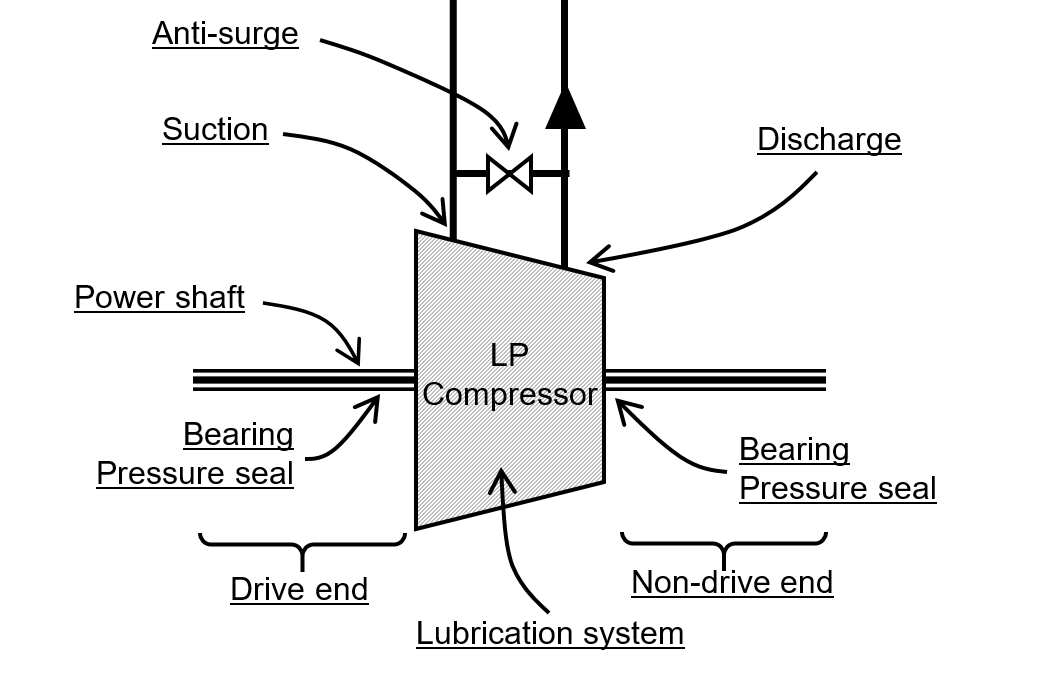
\includegraphics[width=0.7\textwidth]{lp-stage.PNG}
	\caption{A more detailed figure showing sensor location at the compressor.}
	\label{fig:lp-stage}
\end{figure}


\end{appendices}

\newpage
\bibliographystyle{plain}
\bibliography{bibliography}
\end{document}
